\documentclass[journal]{./IEEE/IEEEtran}
\usepackage{cite,graphicx, placeins}

\setcounter{tocdepth}{5}
\setcounter{secnumdepth}{5}

\newcommand{\SPTITLE}{eyeGalaw: A Google Chrome Extension for Webpage Navigation through Human Gaze}
\newcommand{\ADVISEE}{Christine Mae H. Juruena}
\newcommand{\ADVISER}{Katrina Joy M. Abriol-Santos}

\newcommand{\BSCS}{Bachelor of Science in Computer Science}
\newcommand{\ICS}{Institute of Computer Science}
\newcommand{\UPLB}{University of the Philippines Los Ba\~{n}os}
\newcommand{\REMARK}{\thanks{Presented to the Faculty of the \ICS, \UPLB\
                             in partial fulfillment of the requirements
                             for the Degree of \BSCS}}
        
\markboth{CMSC 190 Special Problem, \ICS}{}
\title{\SPTITLE}
\author{\ADVISEE~and~\ADVISER%
\REMARK
}
%\pubid{\copyright~2006~ICS \UPLB}

%%%%%%%%%%%%%%%%%%%%%%%%%%%%%%%%%%%%%%%%%%%%%%%%%%%%%%%%%%%%%%%%%%%%%%%%%%

\begin{document}

% TITLE
\maketitle

% ABSTRACT
\begin{abstract}

% The abstract should be \textit{informational}. Typically a single paragraph
%of about fifty to two hundred workds, the abstract allows your readers to judge
%whether or not the article is of relevance to them. It should therefore be
%a concise summary of the aims, scope, and conclusions of your work. There
%is no space for unnecessary texts; an abstract should be kept to as few words
%as possible while remaining reasonably informative. Irrelevancies, such as
%minor details or a \textit{description} of the structure of the paper, are 
%inappropriate, as are acronyms, abbreviations, and mathematics. Sentences such
%as ``we review relevant literature" should be omitted.\cite{Zobel97}
%

eyeGalaw is a Google Chrome extension that uses eye movements to navigate webpages using an ordinary camera. Functions include  scrolling up and down, back and forward page, hide and show interface,  and enabling and disabling scrolling. Using this extension, the user can normally browse a webpage by clicking and scrolling  and at the same time navigate using eye movements. eyeGalaw offers a new experience in web navigation, and can possibly revolutionize webpage navigation that caters for everyone, even for people with special needs. 


\end{abstract}



% KEY WORDS
\begin{keywords}
eye tracking, webcam, object of interest, navigation
\end{keywords}

% INTRODUCTION
\section{Introduction}

\subsection{Significance of the Study}

The study of eye-movement in cognitive science made its debut during 1970's to 1980's and continued to flourish even up to this date. Eye tracking studies have contributed greatly to different domains such as psychology and neuroscience, medical field, economics, human computer interaction (HCI), and many more \cite{Imotions} but its application to our everyday lives such as market researches, improving user experience in designing products, and health care among others,  only began up until late 2000s. Consequently, eye tracking devices also evolved from pure observation of the eye to huge worn head-devices then evolved  to the smaller pieces of eye tracking devices used today  \cite{Eyesee}.

Studies by Bee \cite{Bee06etal},  Yang  \cite{Yang2016etal}, and  Lee et al.  \cite{Lee2015etal} used the sensor type video camera device for eye tracking. These studies can be a major breakthrough in the area of user experience and usability of applications. However, conducting eye tracking studies like these are limited by the eye tracking hardware. Due to this limitation, Papoutsaki et al. (2016) , have created Webgazer, a JavaScript library that uses an ordinary web camera enabling the further exploration of eye tracking technologies without the use of other physical hardware device \cite{papoutsaki2016webgazer}. This study used an ordinary webcam for eye tracking instead of using eye tracking devices available on the market.

Systems navigated using eye-movements have been well studied and are already being used over the past years. Such technologies include Tobii Dynavox and Samsung’s EyeCan+  which specifically cater for persons with special needs such as aphasia, cerebral palsy, muscular dystrophy, spinal cord injury and many others that has problems with their hands \cite{matos_2010}. But even with the current technology, there are minimal published study yet that uses the web camera in creating systems suitable for these kind of individuals. Using an ordinary webcam, this study  paved the way for web page navigation through human gaze only. This was implemented by creating a Google Chrome extension for the ease of installation and integration to the browser. The result of this study could revolutionize web page navigation that caters for everyone, especially for those with disabilities. 


\subsection{Statement of the Problem}

The eyes, considered as the most strained part of the body, cannot only  be limited to gathering information. Technology has lead us in the age where these gathered information are not merely used for mental processes but as an input in processes that require interaction. However, not everyone, especially people with disabilities can provide the interaction needed for these processes to take place. Devices that are not limited by navigating through touch or mouse clicks expands its usability to people with special needs. This  provided an easier and faster way to perform tasks for most users and enable people with disabilities to use it too. Internet usage all over the world have gone up to almost 40\% percent \cite{hostingfacts.com_2016}, and most of these devices are already connected to it which increases the need for easier web page navigation in devices suited for everyone. This study  focused on navigating web pages using the eyes as a starting scheme in revolutionizing navigation that can be suitable if not for everyone, but even for people with special needs, aiming to improve the efficiency of the overall experience of the users. 


\subsection{Objectives of the Study}
The general objective of the study is to develop a Google Chrome extension that enables navigation on active web pages through eye-movement using an ordinary web camera. The specific objectives of this study are as follows:
\begin{enumerate}
\item to incorporate basic (normal click and scroll) and advanced (gaze controlled) navigation methods;
\item to detect the user’s gaze location on the screen using an ordinary web camera; and
\item to navigate active web pages using eye-movements;
\end{enumerate}

\subsection{Scope and Limitation}
The study focused on navigation on active web pages only using Google Chrome extension on Google Chrome version 47+. This will not consider compatibility to other browsers. To maximize the potential users, Google Chrome is the chosen browser since as of October 2016, Google Chrome has the highest usage having 57.1\% \cite{w3counter_global_web_stats}. Due to the nature of the eye tracking technology used, users were only limited to people who do not need an eye glasses whenever using a computer since eye tracking will be difficult if there is an obstruction on the face. eyeGalaw will not be able to cater to individuals with eye-movement disorders and focusing problems. The Google Chrome extension will always ask for the user’s permission before the web camera will be enabled in the browser. Users will be notified on the start and end of the eye-movement recording. Running the web camera will only be recording the necessary data for the eye tracking. It is not the concern of the study as to how the user will open the browser. Note that extension is only limited to its control functionalities (scroll up/down,next/previous page and hold) thus, clicking through links and other tasks that require interactions should not be affected. 

% RRL
\section{Review of Related Literature}
Among all the information gathered by the senses, 80\% of this is composed of visual information. This is why the eyes are considered as the most important organ among the five senses \cite{gordon_1989}. Knowing how this information are processed by the eye is important in understanding how we perceive. 

A study by Holánová \cite{holánová_hedberg_nilsson_1999} have elaborated characteristics of eye-movement. One of this characteristic is how eye-movements are affected by experiences, choices and personal interest. This characteristic can be seen in the result of a study by Shimojo, et al \cite{shimojo_simion_shimojo_scheier_2003} which presented a model, one of its components called ``preferential looking''. The model explains that the more the person likes an object, the longer the individual looks at it. This characteristic also helped coin the term ``area of interest''. 

The other characteristic discussed in the paper of Holánová et al. is how the eyes play the ``Game of Memory''. This states that eye-movements tend to go faster between objects and spend less time  on the objects they are already familiar with than the objects they see for the first time. This was seen in an experiment by Edwards \cite{edwards_1998} that eye-movements are smoother on familiar objects but shaky on unfamiliar ones (e.g when searching for an object in a screen). In line with the findings of Edwards \cite{edwards_1998}, Bulling and Roggen  \cite {bulling_roggen_2011}  also found the same result in her study that eye-movement analysis showed that unfamiliar faces show more dispersed eye-movement data compared to faces the respondents already know. 

This  research will be stressing of how important it is to study the concepts of ``areas of interest'' in correlation with eye-movements since there will be specific areas on the screen that will be the user’s target of gaze to navigate the website. Understanding the concepts behind this can lead to a better explanation of how the patterns of eye-movement affect in perceiving an object or the whole area itself.

\subsection{Components of eye-movements}

The interplay of factors in eye-movement patterns can be further understood by studying its components. 

\subsubsection {Saccades, fixations, and smooth pursuit}\leavevmode

\paragraph{Saccadic}\leavevmode 

The eyes are known to be always moving unconsciously. These usually unnoticeable quick, erratic eye-movements that jump from one point to another is called saccades. When an image is moved simultaneously with the eye-movement, the image formed in the brain naturally fades due to the “neural adaptation”  \cite{martinez-conde_macknik_troncoso_dyar_2006}. Some studies  by Gerrits and Vendrik  \cite {gerrits_vendrik_1970}, Sharpe  \cite{sharpe_1972} as cited in Martinez-Conde  et al.  \cite{martinez-conde_macknik_troncoso_dyar_2006}, claim that this is where microsaccades, small saccades, are useful, in which it “refresh retinal images” that reduces the effect of the image fading. But past studies conducted during 1970’s counters this argument stating that trained individuals can hide their microsaccades and that microsaccades are normally hidden in tasks that involve heightening of senses such as shooting a gun; and newer studies by Collewijn and Kowler \cite{collewijn_kowler_2008} also supports that the factors involved, more specifically the “role of the retinal transients” that results from microsaccades are yet to be explored more. 


\paragraph {Fixation} \leavevmode

Fixations occur when eye-movements dwell longer on a certain object or area. Perception starts in the range of 40-50 milliseconds (ms) during exposure to object \cite{rayner_smith_malcolm_henderson_2009}. Fixation durations depends on different factors namely “stimulus processing time, relative emphasis on speed or accuracy, sequential dependencies across fixation, and amplitude of the preceding and following saccades”  \cite{salthouse_ellis_1980}. 

Among the most recent promising results involving fixations is a study using Electroencephalography (EEG) and eye tracking that aimed to determine the observer’s choice among the objects on the screen. The study confronted the issue that each of the objects on the screen may have different saliency, the qualities that get the user’s attention, that may result in recognition happening in “peripheral vision”. Other factors like neural process may also be a factor in the delay in the eye-movements. The classification algorithm used in the study successfully determined which object/s were the target of interest of the user and which are not given the variables: saliency of the objects and the “timing of neural activity related to target recognition.” Even with the users’ not being restrained with their eye-movements, the result of the EEG and eye tracking still correlated \cite{wenzel_golenia_blankertz_2016}. 


\paragraph{Smooth pursuit} \leavevmode


Whereas saccades and fixation eye-movement types refer to tracking non-moving objects, smooth pursuit eye-movements follow  a moving object. This study, however, will not tackle eye tracking in moving objects but since it is still a component of eye-movement, discussing it in this chapter will help readers in clearly defining its difference with other components. 

In smooth pursuit, the eye speed is comparably slower than that of a saccade. Saccadic eye-movements are quick and erratic while smooth pursuit  eye-movements are steady and continued eye-movement. Since smooth pursuit are continued eye-movements, tracking an object needs to have continuous feedback too in order to have a clearer image of the object  \cite{chen_choi_2013}. 



\subsubsection{Visual Attention} \leavevmode

Gazing at different locations in a scene does not automatically mean the eye can process the gathered information all at once. The processing of this information undergo two parts, the “recruiting and focusing”. The first one is recruiting, which refers to the collecting of visual attention and resources such as the capacity of a person. This capacity indicates the amount of perceptual resources gathered which is affected by physiological factors such as fatigue and rest, and psychological factors such as alertness, motivation, and time of the day\cite {osman_dupire_mader_cubaud_natkin_2016} . 

The second part is “focusing” that deals more on selecting which object to process among everything the eyes see in a scene in a short span of time. This process of selection can be further classified into two forms. The most common form is the overt selection which is done when a fixation is transferred from one point to another thus, the transfer of attention to the latter point. This is creates the area of interest in which covert selection takes place. However, it is not necessary that the attention is always in the area of interest where an individual is looking. It might be somewhere out of one’s field of vision. This is identified as a covert selection  \cite {hedberg00} \cite{chen_choi_2013} . According Holánová et al.  \cite{holánová_hedberg_nilsson_1999}, as cited by Hedberg  \cite {hedberg00}, what the brain is “actively processing” does not automatically mean it is the image projected on the retina. 

\subsubsection{Definition of Areas of Interest} \leavevmode


According to Hedberg  \cite{hedberg00}, areas with clumped fixations are called areas of interest. It is assumed that attention is focused on the said areas which indicates a visual stimulus from the scene. This will assure the objectiveness of the study since the prediction of the areas of interest will not be solely based on “semantic knowledge” which parts of the scene are considered interesting. 

When measuring fixation data in identifying areas of interest in this study, it should also be noted that there are considerations that should be observed. Larger objects in the scene may have smaller parts inside it and may generate fixation data not so close to each other. Even if this study will not consider the time fixations happened, it is worth noting that Hedberg  considered fixations with different time is but is considered clumped is still within the area of interest \cite{hedberg00}.


\subsection{Eye tracking} 

\subsubsection{Current eye tracking hardware} \leavevmode

Common problems in the past when conducting eye tracking experiments include the cost of the hardware, low quality results (with so much noise and distortion) and the stabilization equipment during recording (Glaholt and Reingold, 2009) \cite {glaholt_reingold_2009}. The strict head positions to be followed to obtain accurate results were very challenging thus the natural and relaxed state of the subject cannot be easily tested (Hedberg, 2000) \cite {hedberg00}. 

Advancement of technology in the past 50 years has addressed these limitations resulting to better eye tracking data. This includes the improvements on data accuracy, real-time data control, and even generation of spatial and temporal eye-movement data have been made possible. 

Present eye trackers include a remote or mounted sensor device, a non-intrusive type of eye tracking that  “directly measures eye line of gaze with respect to a stationary surface” requiring the users to have a fixed head position \cite {choosing_an_eye_trackingSB}.
. 

Remote eye trackers provide the most simple and convenient way to measure gaze on a scene and enable real-time data control. Nevertheless, limitations using this device include the distance of the user to eye tracker and vice versa which will depend on the eye tracker capability. Another is the incapability of  this type in capturing exact data whenever there is much head twist and turns in a multiple field or scene.

Similar to the previous type, the head-mounted eye trackers functions almost the same as the remote sensor device. The main difference with the previous is the sensor’s proximity to the eye of the user and allows more head movement freedom. Similarly, it also measures the eye line of gaze but in contrast to the previous one, with respect to the head. \cite {choosing_an_eye_trackingSB}.

Another common type of eye tracker is an eye glasses with an embedded eye tracker frequently used in tracking eye-movements in a natural environment (e.g., reading a book) which offers broad range of application because of its mobility and ease of use unlike the first two types. \cite {choosing_an_eye_trackingSB}.


\subsubsection{Approach} \leavevmode

Different approaches are used in several eye tracking techniques but this section will only look into methods  that use a specialized sensor video camera to track eye position. This is used in remote and head mounted eye trackers discussed in the previous section.

This approach measures the iris shape in the images captured by the device. Ambient light is a key factor in conducting this kind of experiment since the quality of the captured eye-movement data depends on it. However, problems in capturing data are experienced in scenes with poor light conditions. As a solution, eye tracking devices are embedded with an indiscernible infrared light that is cast  in the user’s eyes. When the eyes are subjected to infrared light, the pupils tend to be highlighted that allows a better detection of eye-movements. There are cases when the pupil appear to be white as an effect of the light source and the eye visual axis lying on a straight line. 

Remote eye trackers require fixed head position to have better eye tracking. It was suggested that to address inconsistences of the data whenever head position changes, two cameras should be used, a wide angled camera to identify person on the screen and the other one to identify the face and maps out its details. Detecting head movements will require two metrics, the measurement of distance of the user’s face and a 3d orientation of the face from the mapped out details of facial data will used \cite {lupu_ungureanu}.

\subsubsection{Gaze controlled navigation }\leavevmode

Being able to navigate without the use of keyboard or mouse has been a product of several technologies mixed together. Speech navigation and gaze navigation are the most famous among others. These technologies are being continuously developed to provide a wider scope of usability of devices.
Since eye tracking in games has not been extensively studied, researchers have gained their interest in this topic hoping to understand more of its mechanics. Gaze navigation and control enables games to understand users more, not only by the gamer’s behavior but through the information offered by the eye tracking input \cite {isokoski_joos_spakov_martin_2009} . Using gaze as an input, games can already choose a path for its storyline \cite{starker_bolt_1990 }  and predicting users behavior and attention in games   \cite{da_silva_prigent_courboulay_2007} \cite{ munoz_yannakakis_mulvey_hansen_gutierrez_sanchis_2011 } , and predicting areas-of-interest type of games  \cite{vickers_istance_smalley_2010}. Serious games (e.g. learning types) has also adapted eye tracking in to use the information to create better game design \cite{ turner_velloso_gellersen_sundstedt_2014 }.
Similarly, eye navigation is widely used in designing effective user experience in many fields especially in the web. According ot Schall  \cite{schall_2014} this is particularly useful in optimizing navigational elements  and understanding users’ eye path to create a more dynamic content for the readers \cite{marcus_2015}.
The increasing use of the Internet has also brought a bigger need to extend its accessibility to everyone. To achieve this, browsers also need extend its usability to everyone. Gaze navigation can be an integral part in achieving this, allowing motor impaired individuals to also use the Internet through these kinds of browsers. Porta and Ravelli  \cite {porta_ravelli_2009} have developed an eye controlled Web browser that allows page navigation and link selection. Comparably, GazeTheWeb browser, with more features and better functionalities, is closer to browsing using keyboard and mouse. This browser claims to address to more specific types of motor disabilities (e.g Parkinson’s disease, Neuromuscular Disease, and High Tetraplegia) \cite {mamem_2015}. This kind of browsers may offer advantages that current browsers do not have which can be used by everyone specially tailored to a specific group of people. But statistically speaking, these kinds of browsers may not sustain for a long period of time because of low number of users. Ideally, since there are already existing browsers with the same functionalities, adding the eye tracking capabilities done by a standalone web browser to an already existing one is a more efficient way to do it. 
Instead of creating a browser, this study  created a Google Chrome Extension similar to the study of Almazar and Recario; Ventocilla and Recario  \cite {almazar_recario_2016}, \cite{ ventocilla_recario_2014 } that employed web speech navigation using Google Chrome Extension. Google Chrome was the chosen browser to maximize the potential users since it is dubbed as the most used web browser in October 2016 and has been at the top since 2011. Browser extensions is a better choice because it’s a lightweight program that can change functionalities of a web browser allowing for more control in creating the gaze controlled navigation extension.


\subsubsection{Webcam for eye tracking} \leavevmode

Using webcam in eye tracking is a relatively young approach in studying eye-movements. Only a handful, however,  are published online. 

A study explored different “illumination recognition techniques” in facial detection paired with eye tracking in creating an efficient algorithm to obtain user’s gesture in a screen. The algorithm used in the study created a system that uses facial recognition and eye tracking as the main control using a webcam only \cite {lin_chao_lin_chen_2005}.

TurkGaze uses a simple webcam for saliency prediction that offers a cheap and less effort way of gathering data through the webcam. This employed a large scale gathering of data using crowdsourcing. The data gathered from the webcam showed comparable results from the data gathered through usual eye tracking device \cite { guillotel_nguyen_chamaret_fleureau_2013}. 

Another study proposed a saliency based method to distinguish areas of interest in an indoor setting. The study identified the location of salient objects in a scene by mapping the extracted user’s interest points. This indicates that the system can be a cheap way in locating multiple objects in a scene which can be applied in robot navigation and security surveillance cameras \cite{rudinac_jonker}.

A similar research explored on eye gaze analysis on sequences of images in generating a method for calibration free gaze tracking  \cite { guillotel_nguyen_chamaret_fleureau_2013}. PACE, a system that collects “user interaction events” using a webcam created an auto calibrating eye tracker  \cite { huang_kwok_ngai_chan_leong_2016}. 

Among all eye tracking studies listed above, Webgazer, the study of Papoutsaki et al.  \cite{papoutsaki2016webgazer} showed the most promising result of using the webcam in eye tracking. Written entirely in javascript, Papoutsaki et al. created an eye tracking library that used an ordinary webcam to locate eye gaze locations in real-time.

Webgazer features include swappable components for eye detection and multiple gaze prediction models. The researchers provided several javascript library 000000000000000for the users to choose from. These include clmtracker.js library which  tracks head and eye positions. This is a javascript library for fitting facial models to faces in videos or images. It tracks a face and outputs the coordinate positions of the face model as an array, following the numbering of the model of points plotted as a facial lines \cite{auduno-clmtrackr}. Another library used is js\_objectdetect, a javascript library for real-time object detection, tracking,  and for various augmented reality applications that run in the browser without any plugin \cite{js-objectdetect}. Webgazer used this to capture face and eye positions. Trackingjs library was also included in this list. This library incorporated different computer vision algorithms and techniques to enable to do real-time color tracking, face detection,  and many more \cite{lundgren}. Webgazer used this in order to find the head and eye positions. For the predicition of eye patches, several libraries were also used. This includes LinearReg.js which uses pupil detection and simple linear regression to predict gaze from eye patches, and varieties of RidgeReg.js which uses ridge regression to correlate click and mouse movement to eye patch features  \cite{papoutsaki2016webgazer}.

Due to its novelty, the emerging potential in exploring Webgazer in extending its application in detecting the users’ object of interest can contribute to the limited knowledge of using webcam in eye tracking. The knowledge produced in this study can substatially  contribute to developing further as to how an ordinary webcam through eye-movements can be turned as a navigation tool for web applications developed in the future. 

\section {Methodology }

This study aims to navigate web pages using eye-movements. To address this, A Google Chrome extension was developed as the tool for the navigation of the Web browser. The system and functional requirements, software development process and conceptual framework needed for the development of the Google Chrome extension is discussed in this section. 
\subsection{ System requirements}  \leavevmode
The following tools were needed for development:
\begin{enumerate}
\item HTML 5 and CSS: HTML 5 and CSS, the two core technologies in building web pages, \cite{htmlcssw3c} was  used for the basic layout and designing of the interface of the web extension.
\item Javascript: Javascript is the scripting language used by web browsers. This is the backbone in developing the  extension.
\item Webgazer.js: A real-time eye tracking Javascript based library that processes the input from the web camera will be the middleman between the user and the web browser. 
\end{enumerate}
 


\subsection  {Functional Requirements}
The main functionalities of the Google Chrome extension is listed below:
\begin{enumerate}
\item Settings Tab
\newline
It can be opened by left clicking the icon on the extensions tab on Google Chrome. The following settings can be adjusted: 
\begin{itemize}
\item Scrolling speed
\item Opacity 
\item Enable/disable eye video feed
\end{itemize}



\item Scroll Up and Down
\newline
This enables the user to scroll up or down through the web pages.  The scrolling speed can be adjusted in the settings.  Continuously staring at the  arrows will respond by scrolling at the designated direction. To stop the scrolling, the user needs to gaze at other places on the screen, remove the gaze from the arrows. This is also applicable to all the buttons on the interface. 

\item Back page and Forward page 
\newline
This works similarly like the back page and forward page button in the browser.

\item Hold 
\newline
This lets the user to stay at the current part of the screen without hiding the interface. The hold button can be toggled on or off. Toggling the 'Hold' button  temporarily disables the Scroll Up and Down button, Back page and Forward page. If toggled on, the scrolling of the the web page will be disabled so that the web page will stay at the particular part of the screen even if the user accidentally gazes at the scroll up or down button. The transparency of the interface will be increased to indicate that the interface is temporarily disabled.


\item Toggle Hide/Show interface 
\newline
This permits  the user to hide or show the interface on the browsed web page. 
The button is  labeled 'Hide' while the interface is shown; when hidden, it is labeled 'Show'. As a default, the interface is shown therefore the button will be labeled 'Hide' when the extension is started. 
\end {enumerate}

\subsection {Installation and Activation}
There are two ways to install the extension. The first one is by dragging the .crx file (Google Chrome’s extension file type) to the Google Chrome extensions page found on chrome://extensions. Due to security reasons, the extension might be banned by Google Chrome   detecting it is not from the Chrome Web Store. Instead, enabling the developer mode might solve this problem \cite{ chrome_ext_2014 }.
Clicking the extension's icon  shows a pop-up. Clicking 'Start'  asks for the user's permission to access  the computer's web camera. This is a part of Google Chrome's security feature. When access is permitted, the extension  then adds the external script into the active web page. Injecting the script instead of automatically loading it enables the script to be loaded on the active web page only, giving the user more control over the extension \cite{ dimacali_danila_2016}  \cite{giant_robots_2015} \cite{ marcus_2015 }.
When the extension is started, it loads the interface with its default settings while already getting input from the webcam at real-time. Note that the interface is made adaptive according to the monitor’s screen size. For the interface to work, the browser needs to be maximized first before it will be enabled. The interface will be adaptive for five screen resolutions only chosen from the top screen resolutions used as of January 2016 \cite{w3counter_global_web_stats}. The chosen screen resolutions consist of 1024x768 pixels or higher, namely: 1366x768, 1920x1080, 1280x1024, 1280x800, and 1024x768 pixels. 

Before enabling the interface buttons, an initial calibration phase is required. A loading screen will show up asking the user to click anywhere while looking at the mouse pointer. This is  the user's guide for initially calibrating the click and gaze method for it to increase the accuracy of the prediction of the gaze point. The loading screen  only disappears when eyeGalaw has gathered enough data to predict the user's eye gaze showing the red dot on the screen. In order for the buttons to work, the buttons need to be gazed at a minimum of 4 seconds. This is based on empirically determined value by  Shimojo et al. (2003). Although real-time processing of eye-movement data is done by the WebGazer.js, the accumulation of gaze points at certain buttons still needs to attain a certain number of gaze points before it returns a result where most of the gaze point data are located. Normal clicking of links while browsing will also serve as the calibration to help the prediction of gaze point to be accurate while browsing a page. As stated previously, to stop the currently executed command (i.e.,  during continuos scrolling, going to the next page continuously) the user needs to gaze at other places on the screen, removing the gaze from the previously gazed buttons.  This is applicable to all the buttons on the interface. Note that extension is only limited to its control functionalities (scroll up/down,next/previous page and hold) thus, clicking through links and other tasks that require interactions should not be affected. This click and gaze behavior recalibrates the data, helping the predictions of gaze points become more accurate due to the nature of the used eye tracking library, WebGazer \cite{papoutsaki2016webgazer}. 

\section {Results and Discussion }
\subsection {Chrome Extension}



%{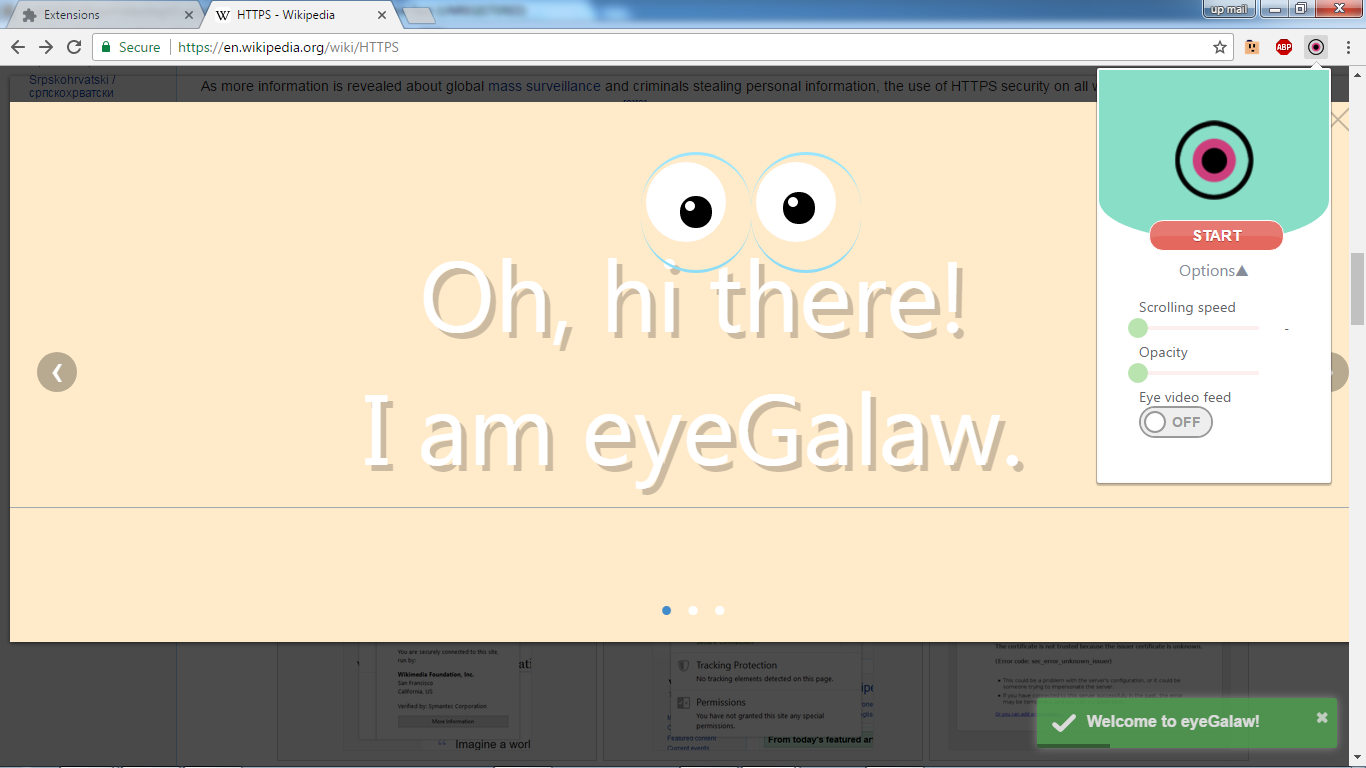
\includegraphics{./images/Fig1.png}}
%{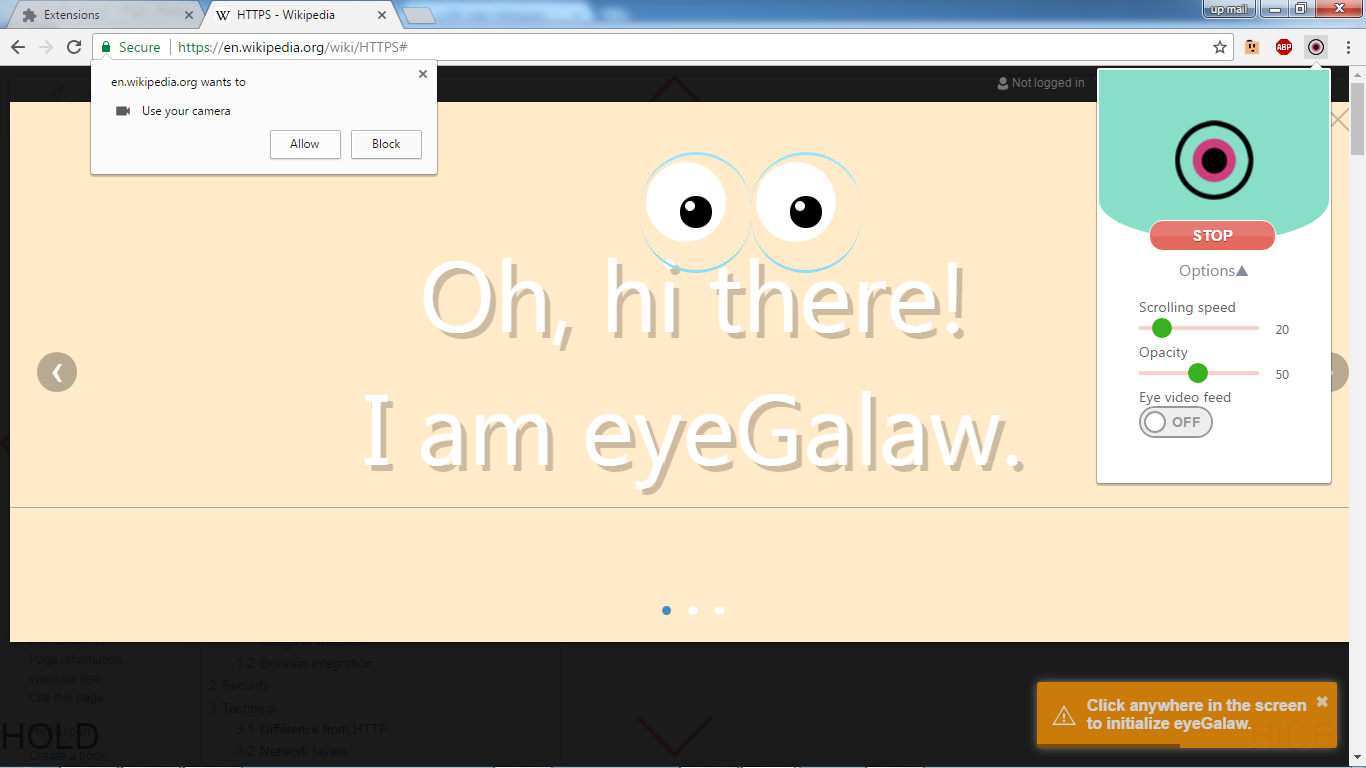
\includegraphics{./images/Fig2.png}}
%{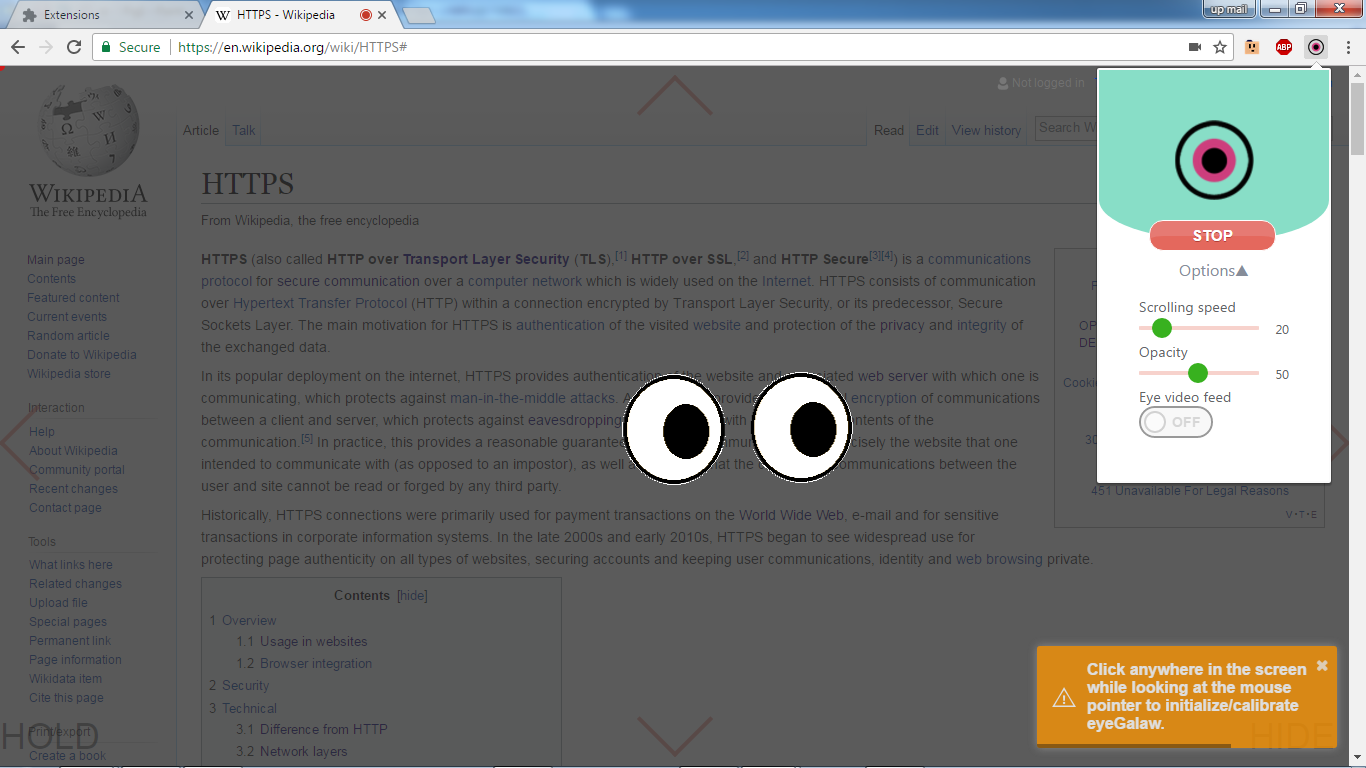
\includegraphics{./images/Loading_screen.png}}
%{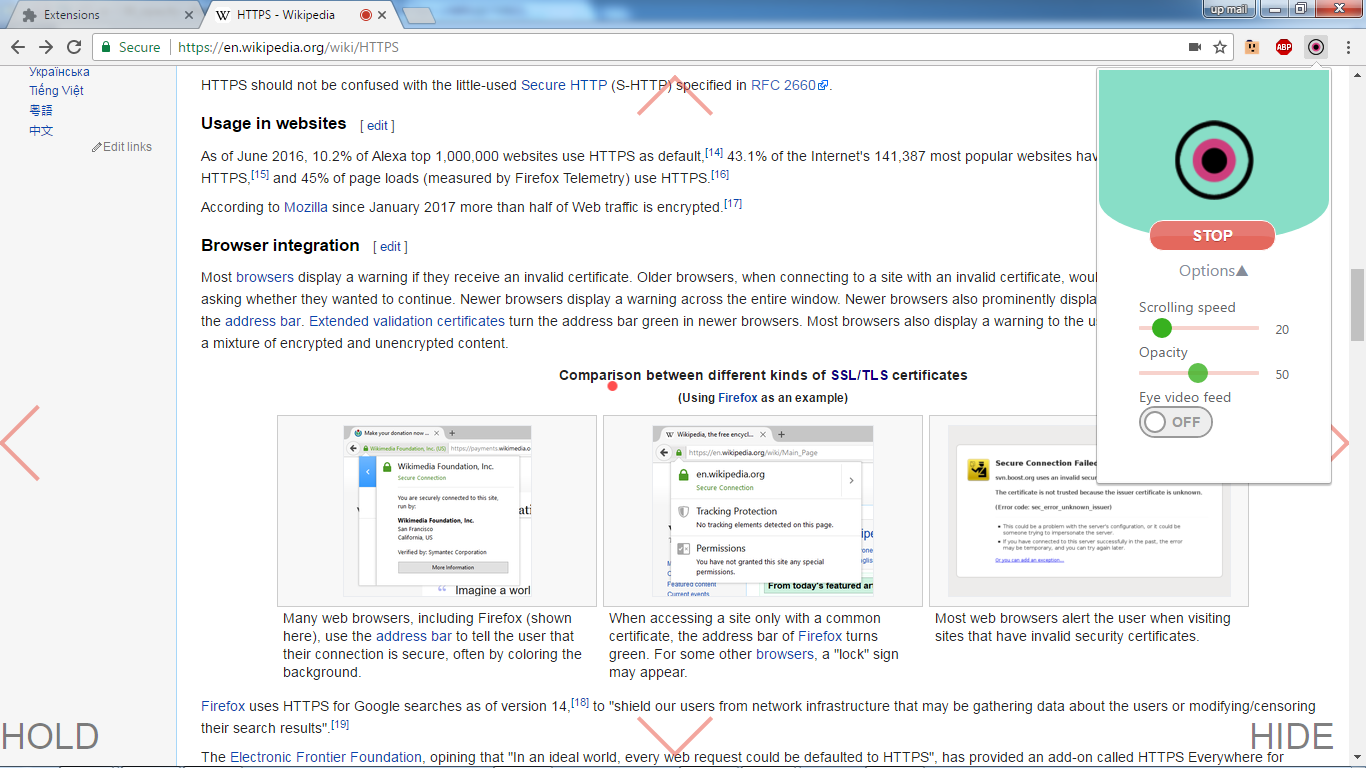
\includegraphics{./images/50_opacity.png}}
%{\includegraphics{./images/100_opacity4.png}}
%{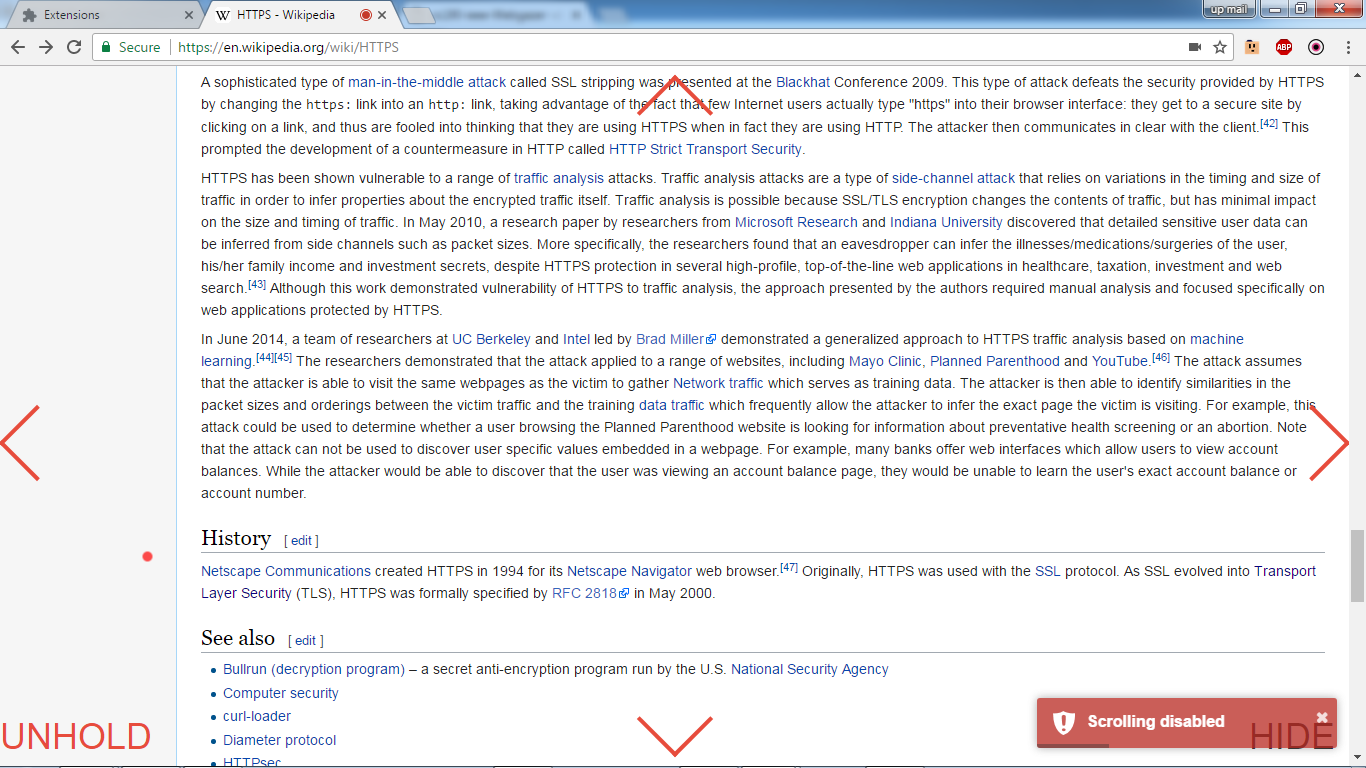
\includegraphics{./images/holded.png}}
%{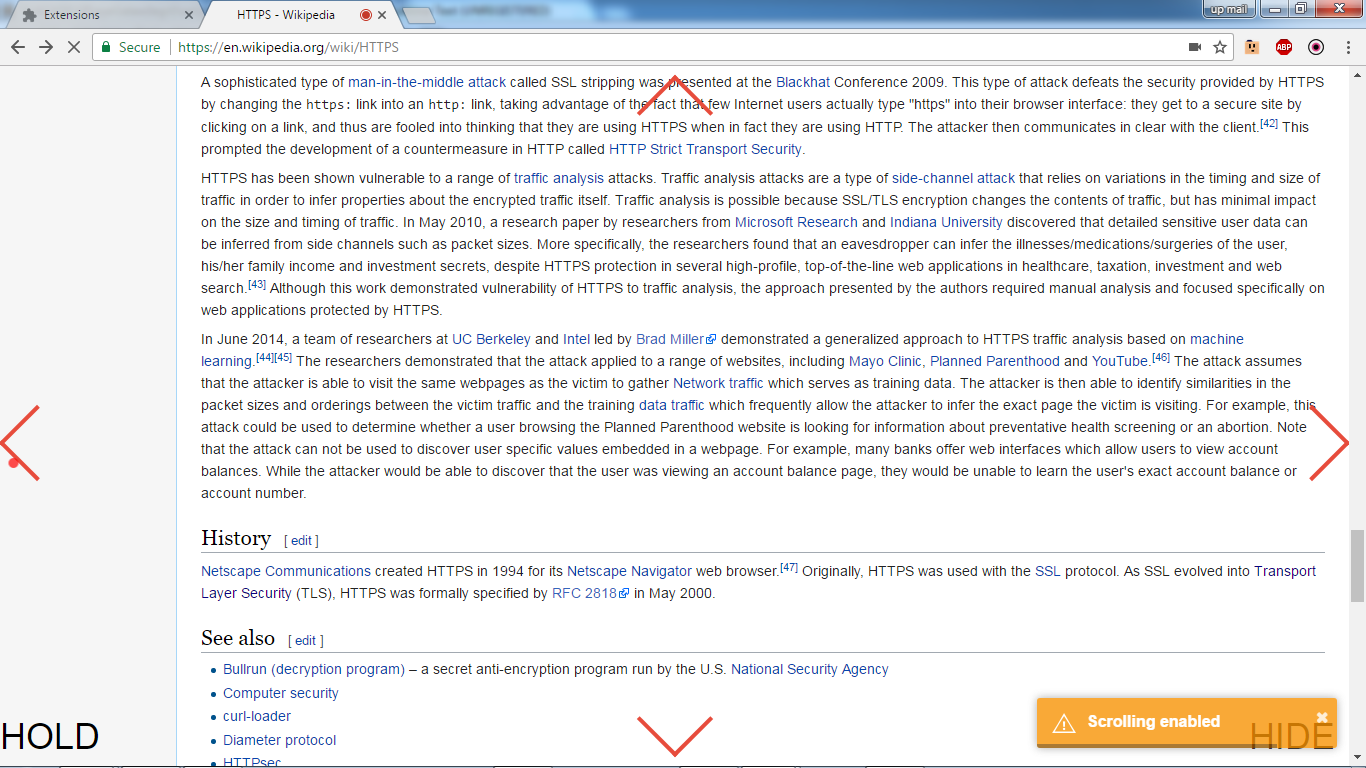
\includegraphics{./images/unholded.png}}
%{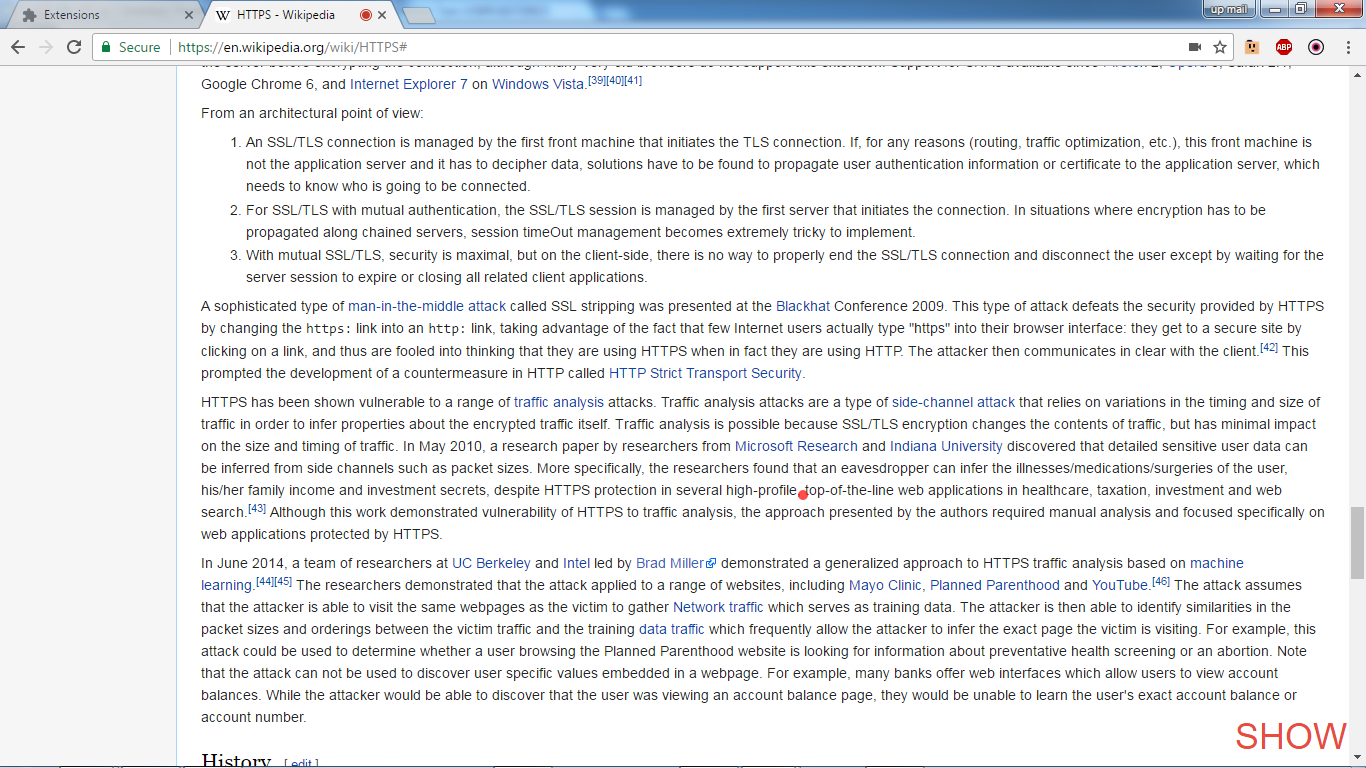
\includegraphics{./images/hidden.png}}
%{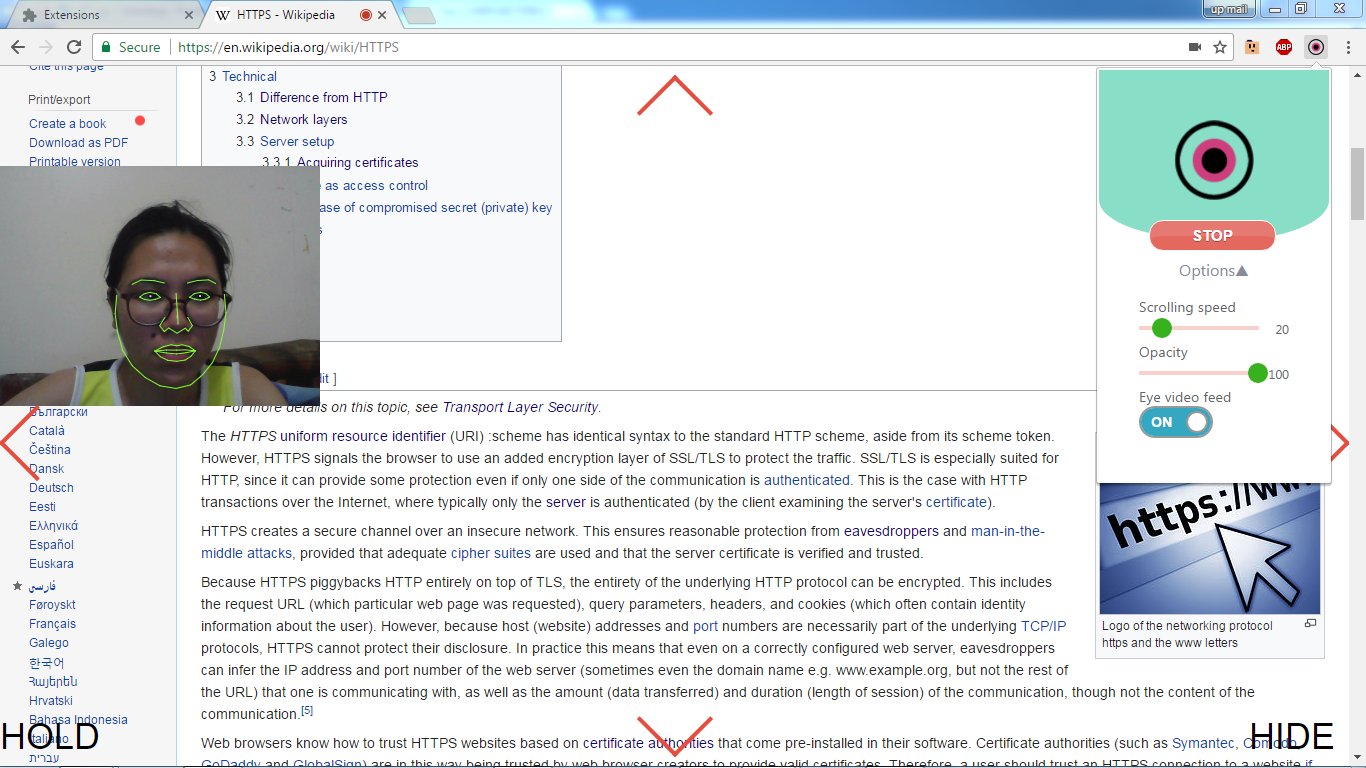
\includegraphics{./images/webfeed.png}}

\begin{figure}[h!]
  \centering
    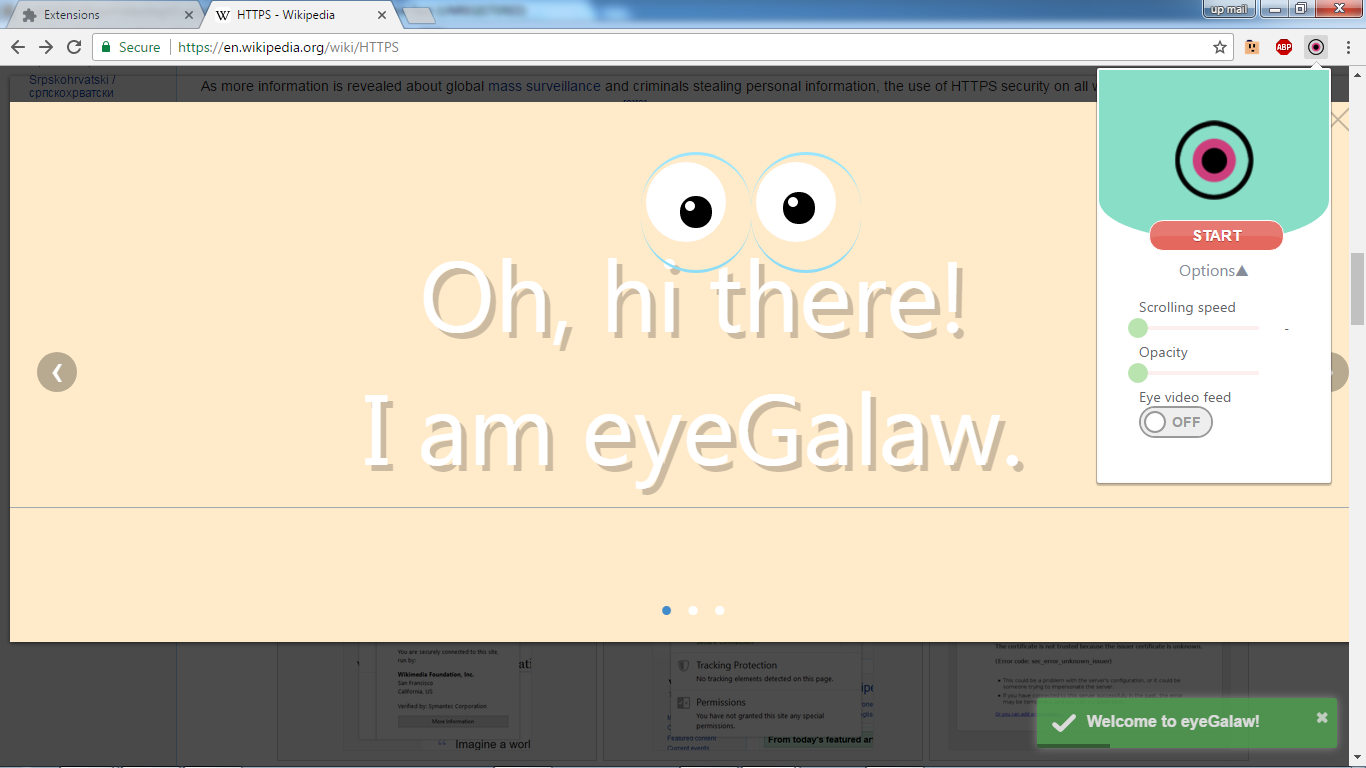
\includegraphics[width=0.5\textwidth]{./images/Fig1.png}
  \caption{eyeGalaw welcome page}
  \label{fig:1}
\end{figure}

\begin{figure}[h!]
  \centering
    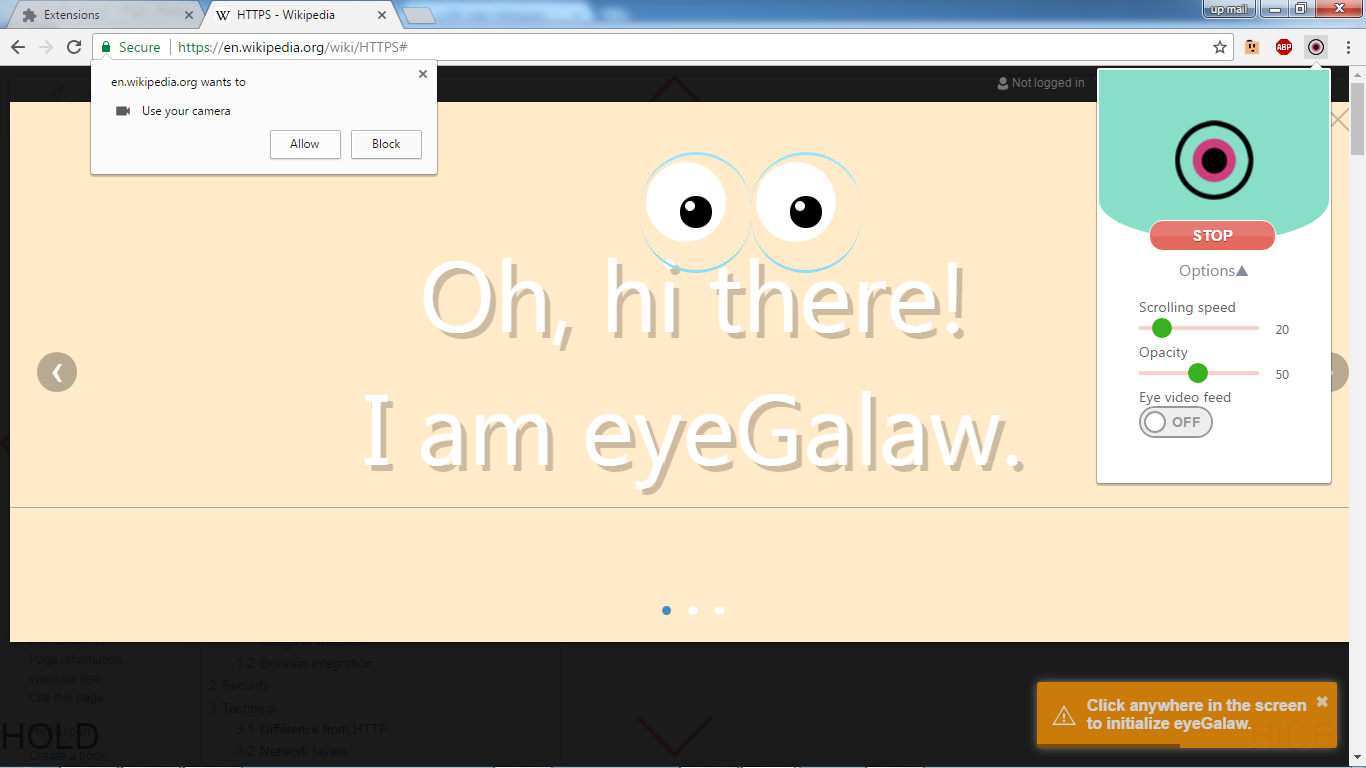
\includegraphics[width=0.5\textwidth]{./images/Fig2.png}
  \caption{Google Chrome's website permission to allow webcam }
  \label{fig:2}
\end{figure}

\begin{figure}[h!]
  \centering
    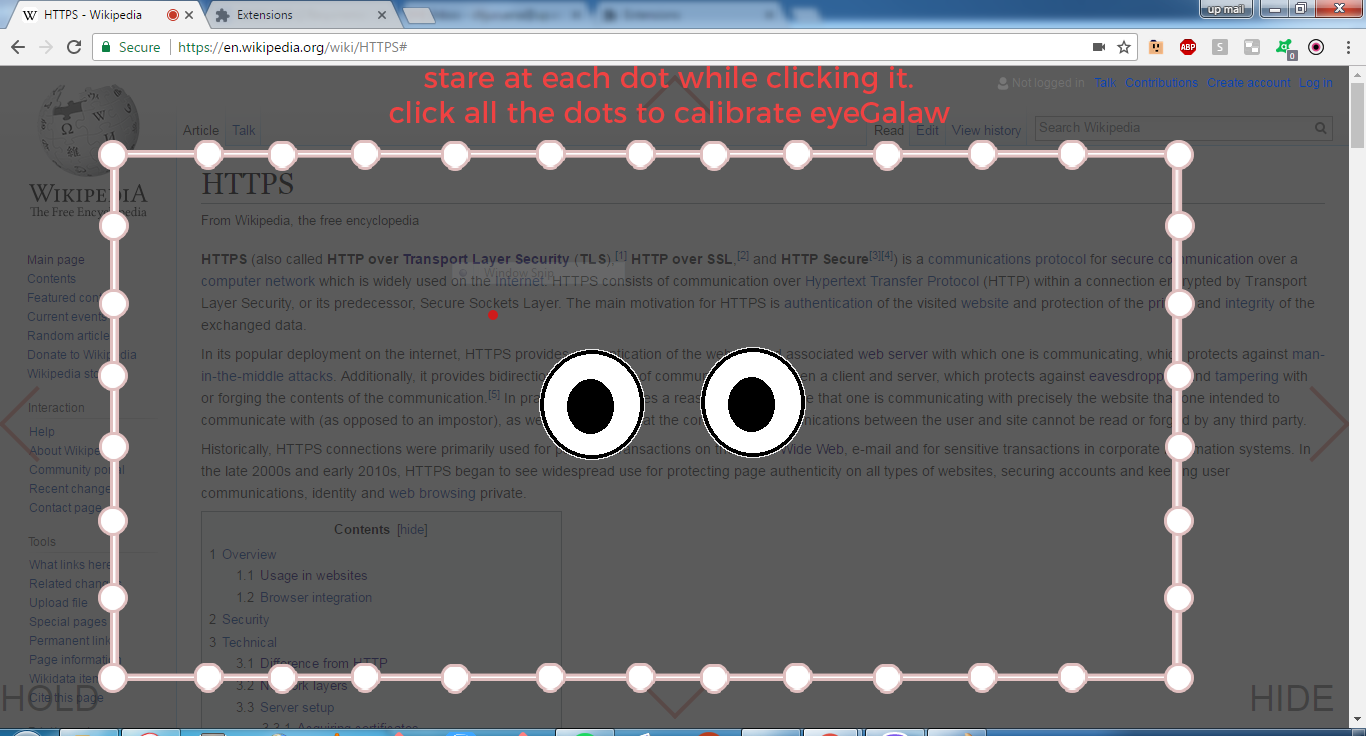
\includegraphics[width=0.5\textwidth]{./images/calibrate.png}
  \caption{Loading screen whenever eyeGalaw needs click-gaze calibration}
  \label{fig:3}
\end{figure}

\begin{figure}[h!]
  \centering
    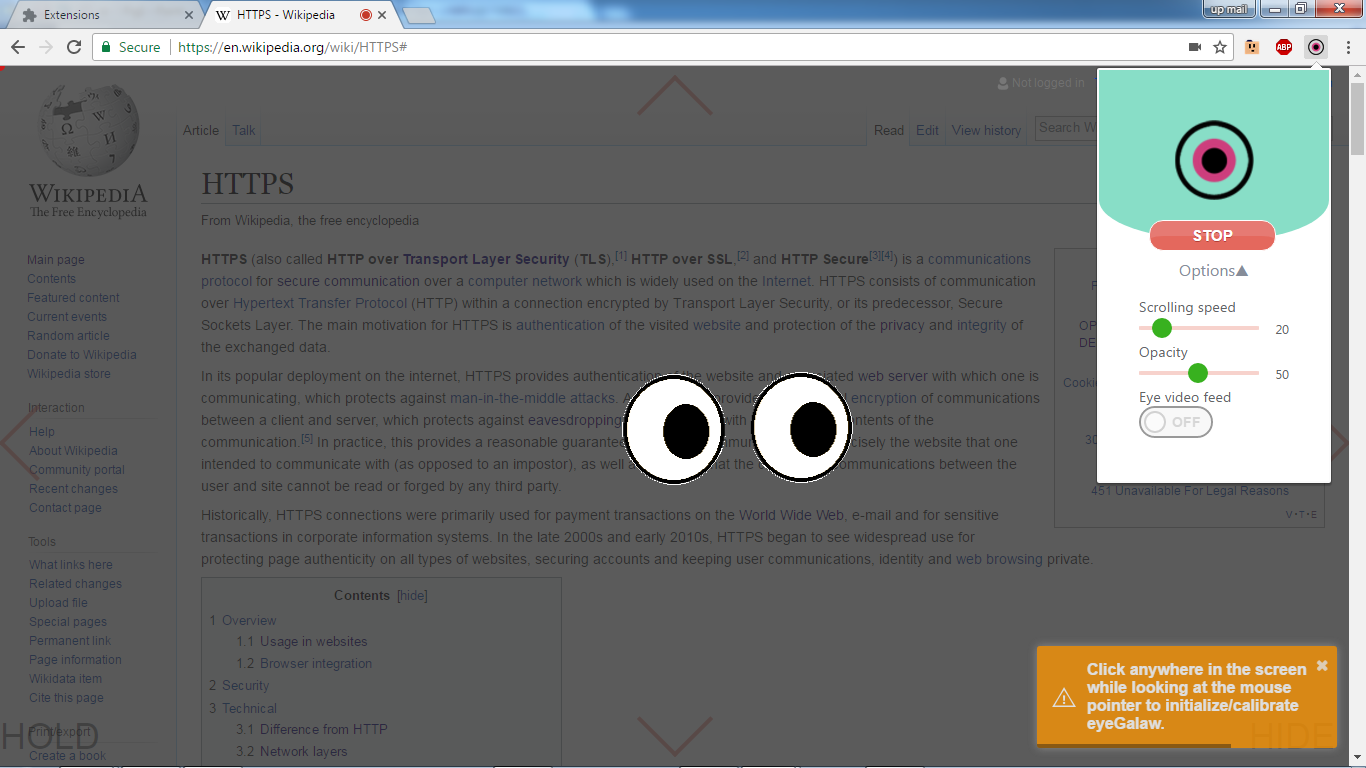
\includegraphics[width=0.5\textwidth]{./images/Loading_screen.png}
  \caption{ eyeGalaw loading screen}
  \label{fig:4}
\end{figure}

\begin{figure}[h!]
  \centering
    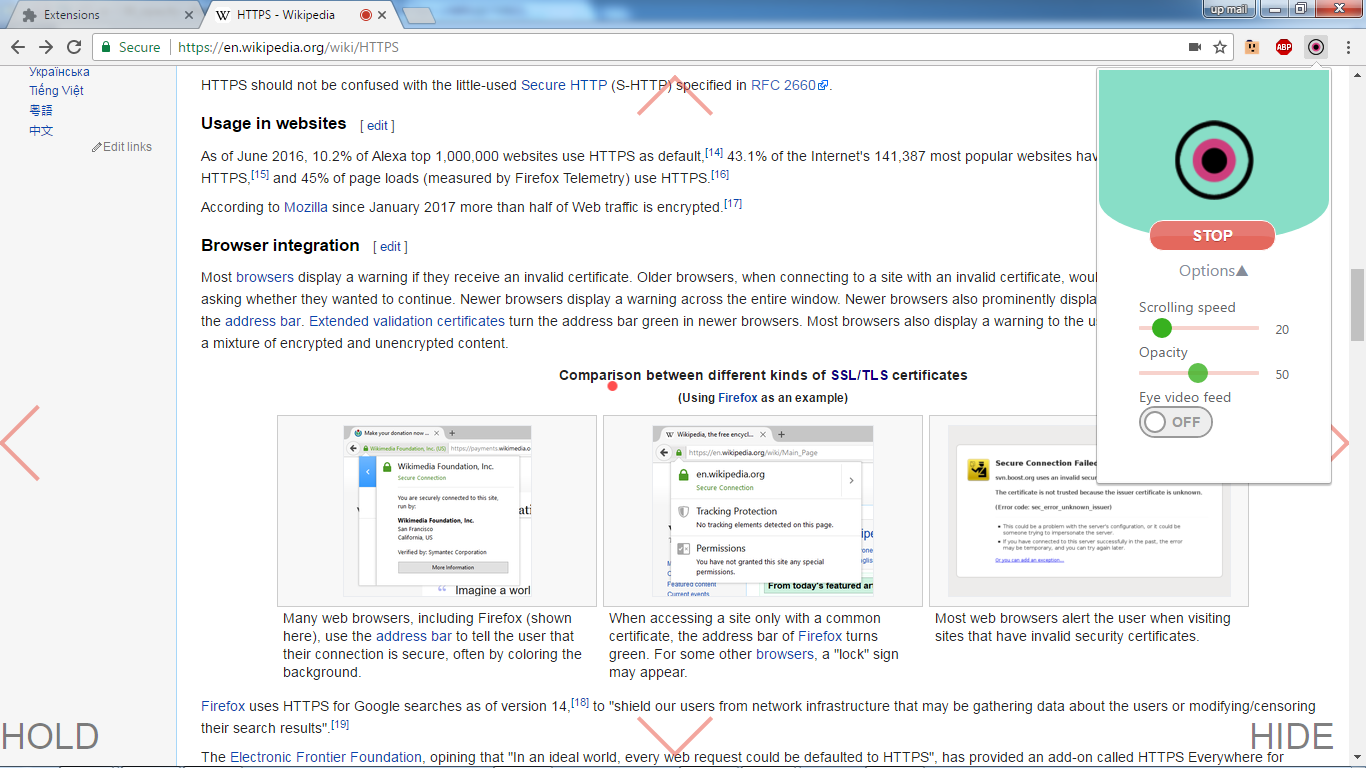
\includegraphics[width=0.5\textwidth]{./images/50_opacity.png}
  \caption{ Default opacity in 50\% }
  \label{fig:5}
\end{figure}

\begin{figure}[h!]
  \centering
    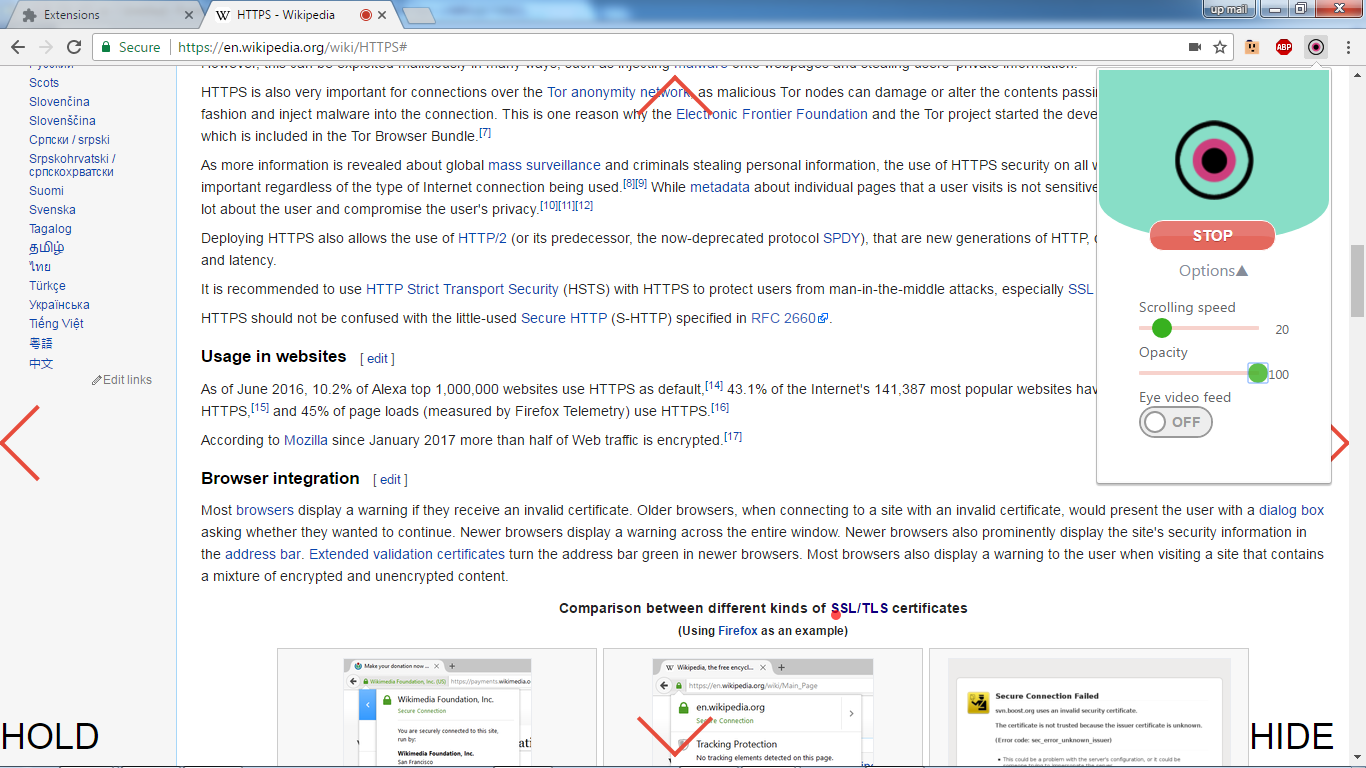
\includegraphics[width=0.5\textwidth]{./images/100_opacity.png}
  \caption{100\% opacity}
  \label{fig:6}
\end{figure}

\begin{figure}[h!]
  \centering
    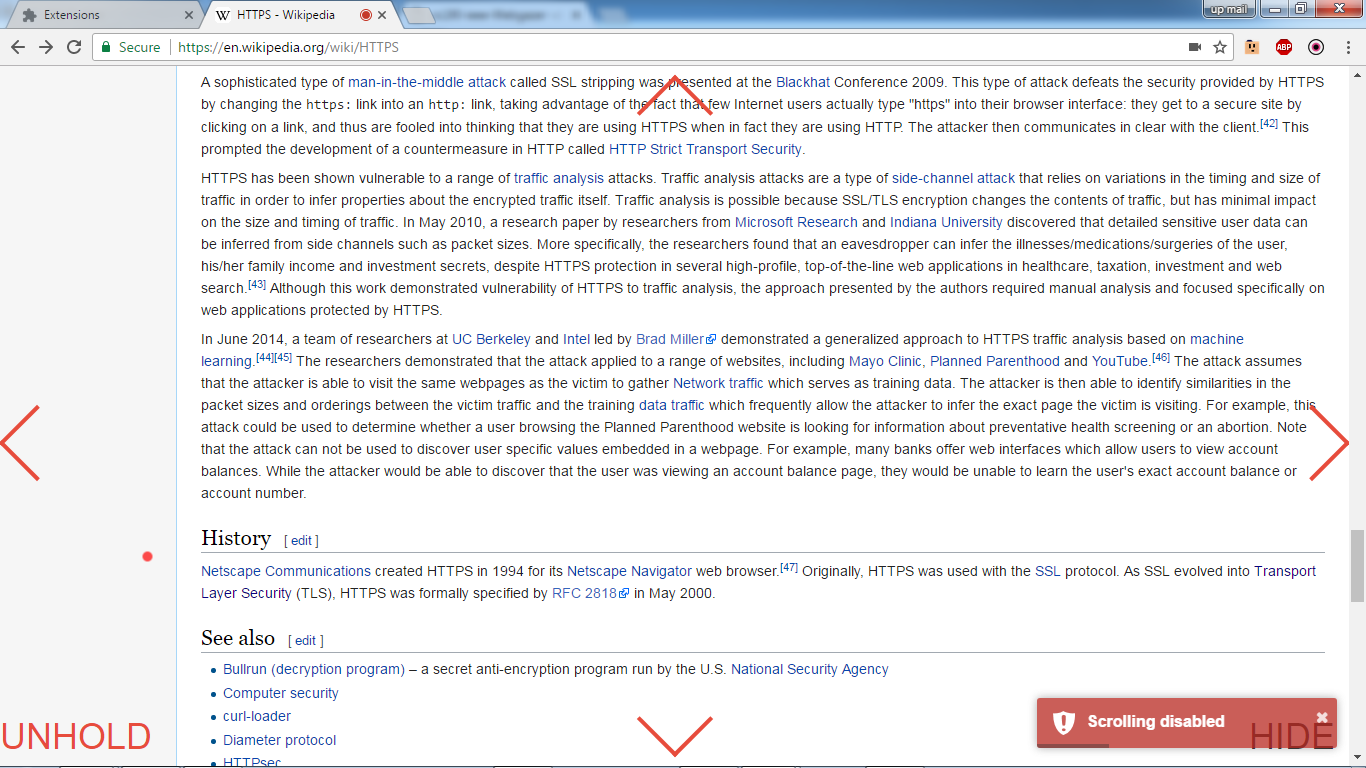
\includegraphics[width=0.5\textwidth]{./images/holded.png}
  \caption{HOLD button enabled, disabled scrolling}
  \label{fig:7}
\end{figure}
\begin{figure}[h!]
  \centering
    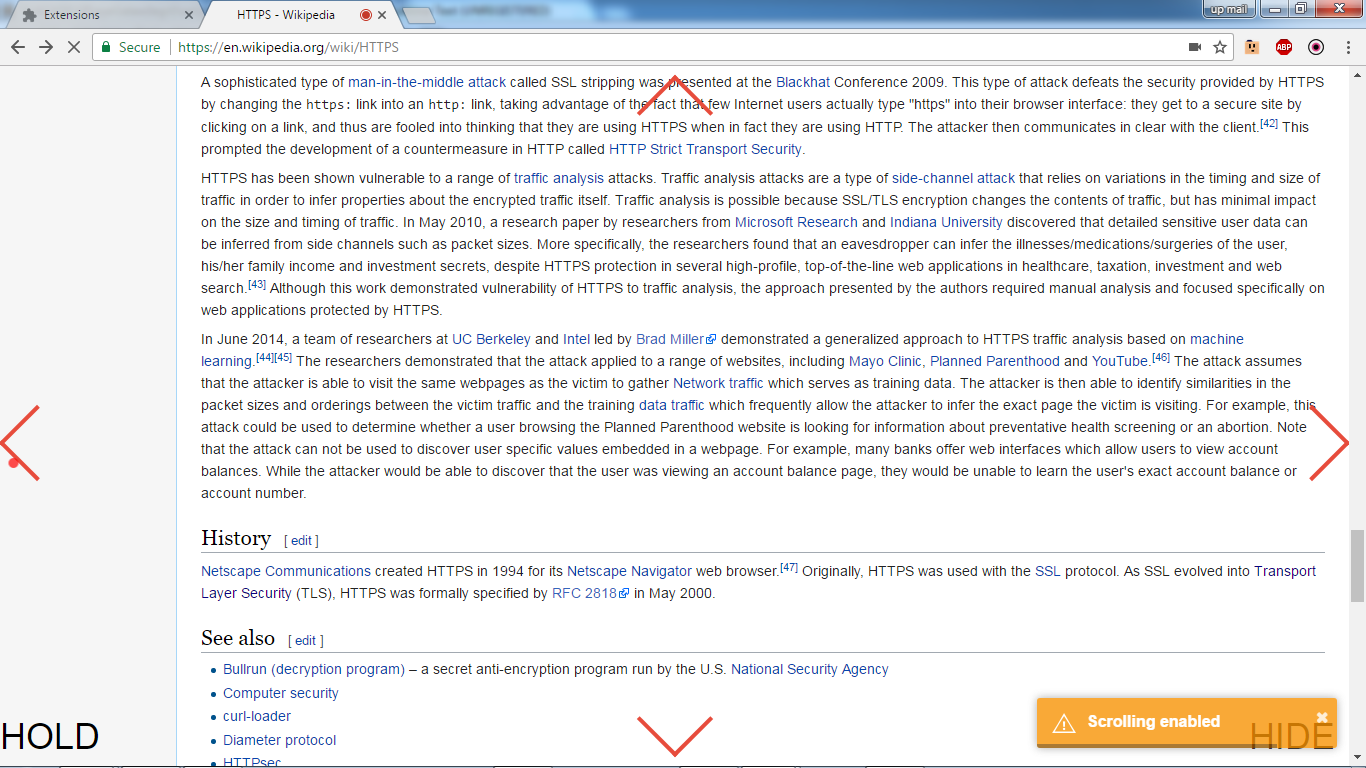
\includegraphics[width=0.5\textwidth]{./images/unholded.png}
  \caption{HOLD button enabled, enabled scrolling}
  \label{fig:8}
\end{figure}
\begin{figure}[h!]
  \centering
    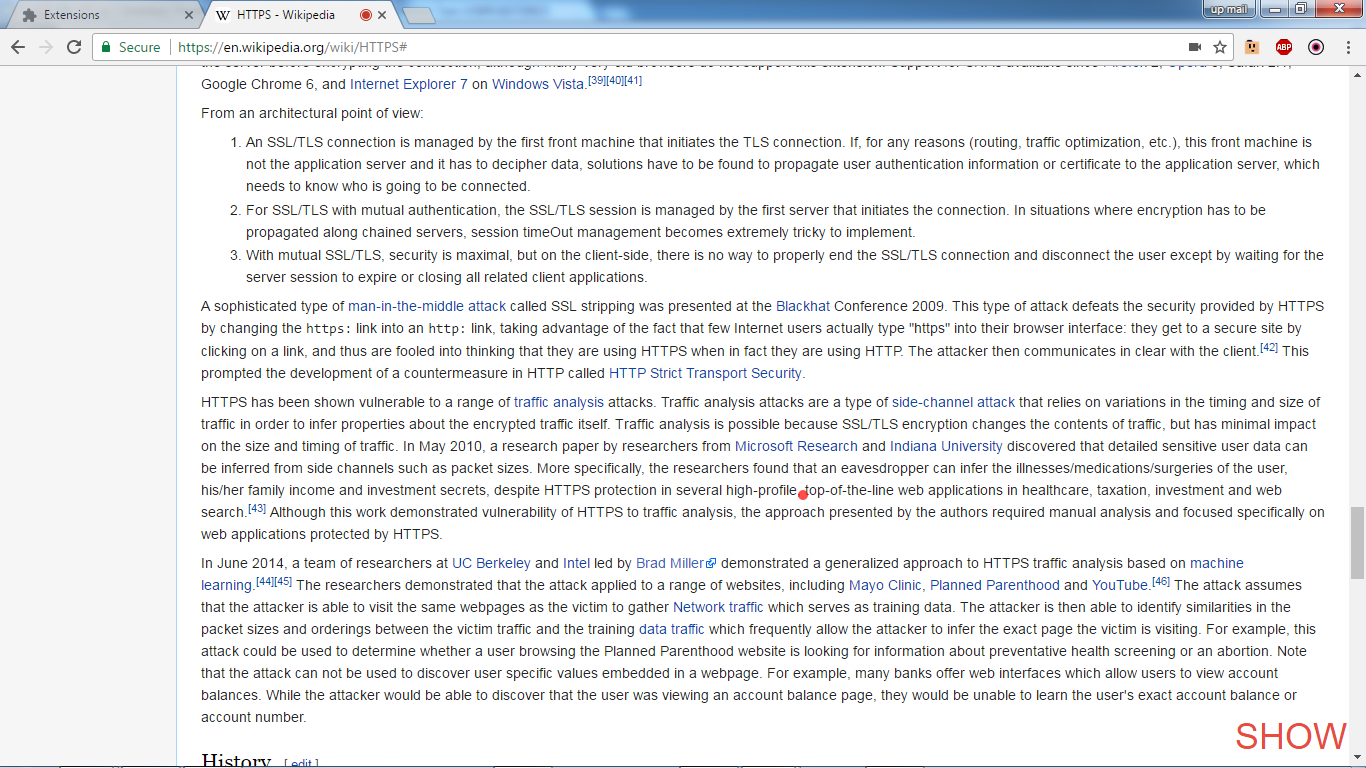
\includegraphics[width=0.5\textwidth]{./images/hidden.png}
  \caption{HIDE button enabled, hiding all the control except itself}
  \label{fig:9}
\end{figure}
\begin{figure}[h!]
  \centering
    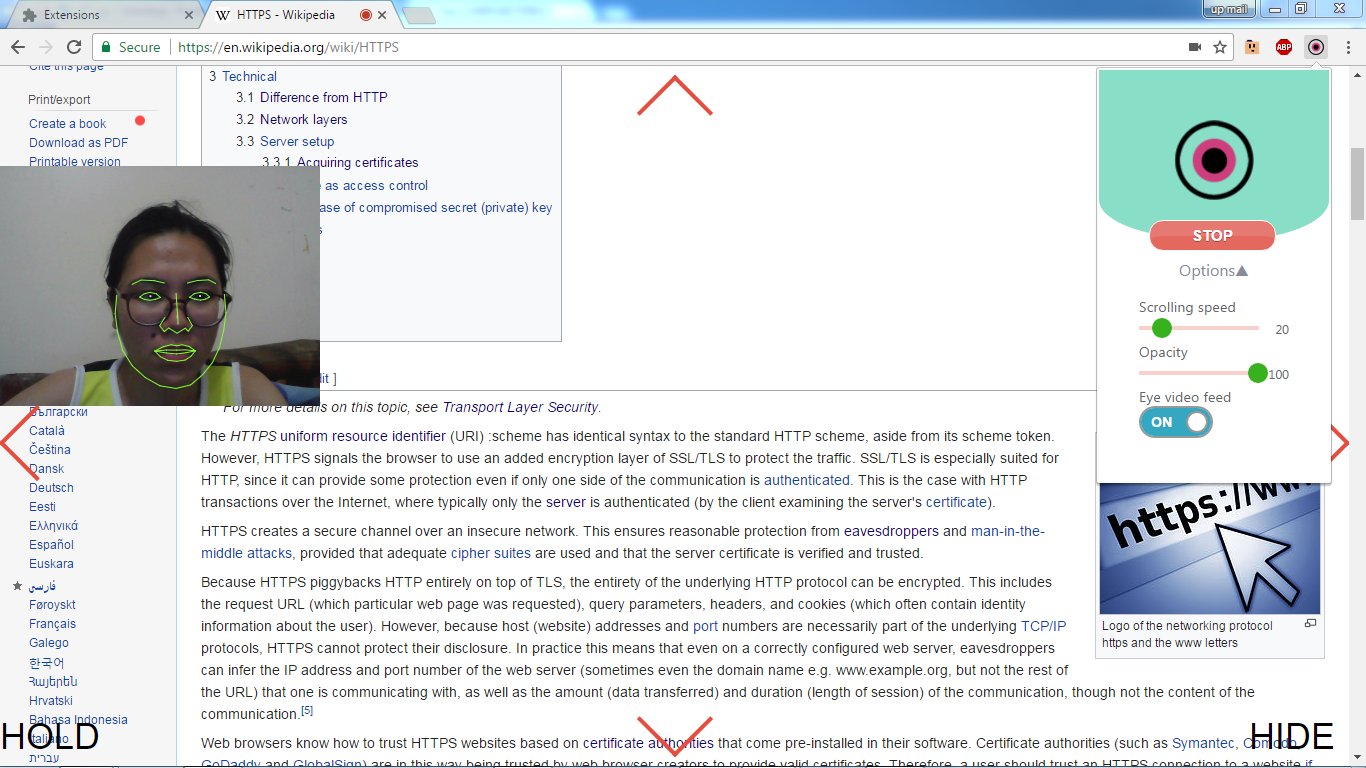
\includegraphics[width=0.5\textwidth]{./images/webfeed.png}
  \caption{Eye video feed enabled, to adjust light and camera angle}
  \label{fig:10}
\end{figure}

A google chrome extension was developed to navigate using the eye movements. The user's gaze location on the screen was successfully detected using an ordinary webcam (see Figure ~\ref{fig:2}). The chrome extension incorporated basic navigation such as normal click and scroll with the gaze controlled navigation method.

Eye gaze input was successfully handled and processed using the eye tracking library Webgazer. At every start of the session, calibration of eye and gaze points is done by clicking all the dots on the screen (see Figure ~\ref{fig:3}). After completing the desired amount of click points, this calibration page will be removed and the user can already start browsing. The normal clicking of links within the browser while browsing a webpage serves as the calibration procedure. Webgazer's real time eye tracking model maps the eye features and click positions on the screen to predict eye gaze location, which is done by looking into the mouse pointer while clicking anywhere in the browser. X and y coordinates of the eye gaze location on the screen was recorded so that when the eye gaze point lands on the certain location, the functionalities (scroll up/down,next/previous page and hold) is activated or deactivated (see Figures~\ref{fig:5}-~\ref{fig:10}).

Since the ex
ension is designed for navigating active web pages, it requires stable internet connection. As a security protocol when webcam access is needed, only secure websites served via HTTPS were allowed to be browsed using eyeGalaw. 

\subsection {Testing}

Using convenience sampling, the extension was tested on different websites by 30 UPLB students from different degrees. After testing, they answered a modified Questionnaire for User Interface Satisfaction (QUIS) by \cite   {lewis_1995} and Computer System Usability Questionnaire (CSUQ)  by \cite  {chin_diehl_norman_1988}.

Analysis of data was interpreted using Top two box (78\%) scoring, which means that the score was evaluated as satisfactory if a score falls within the top two box and a score falling in the middle category is considered as a neutral response between not satisfactory (bottom two box)  and satisfactory (top two box) \cite{interpret_survey_responses}.

The QUIS is composed of four sections evaluating the following: the terminology used and system information, learning how to use the extension, system capabilities, and the overall reaction to the extension. The survey questions are to be rated from 1 (being the most negative reaction to the question) to 5  (being the most positive reaction to the question). Average median  scores of the questions under the said sections were computed (see Figure ~\ref{fig:11}).  
%{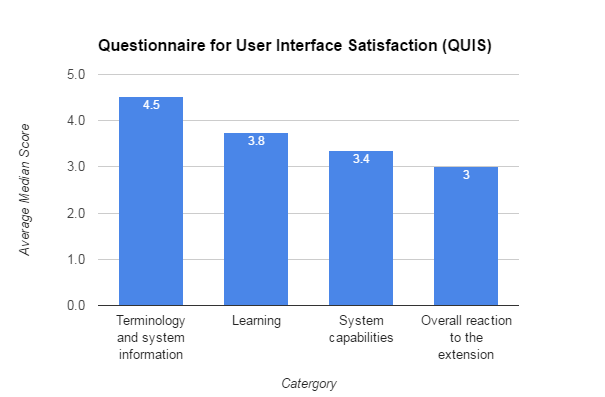
\includegraphics{./images/QUIS.png}}
\begin{figure}[h!]
  \centering
    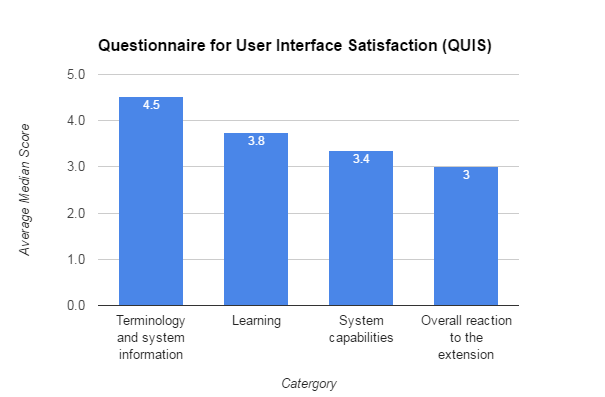
\includegraphics[width=0.5\textwidth]{./images/QUIS.png}
  \caption{Average median  score per section in QUIS }
  \label{fig:11}
\end{figure}
\FloatBarrier
%{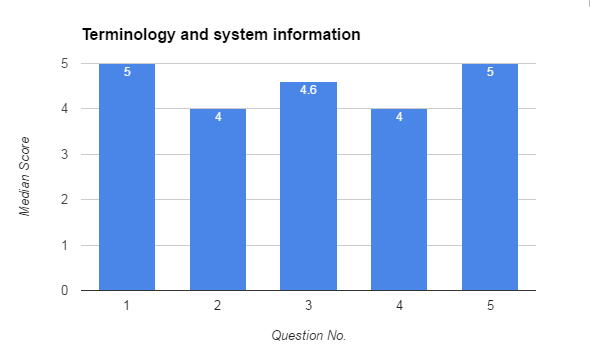
\includegraphics{./images/section1.png}}
\FloatBarrier
\begin{figure}
  \centering
    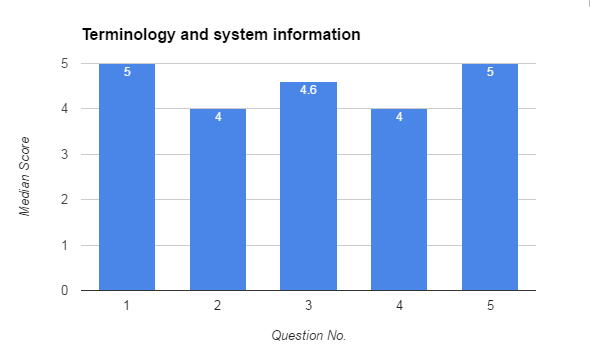
\includegraphics[width=0.5\textwidth]{./images/section1.png}
  \caption{Median score per question in terminologies used and system information section}
  \label{fig:12}
\end{figure}

%{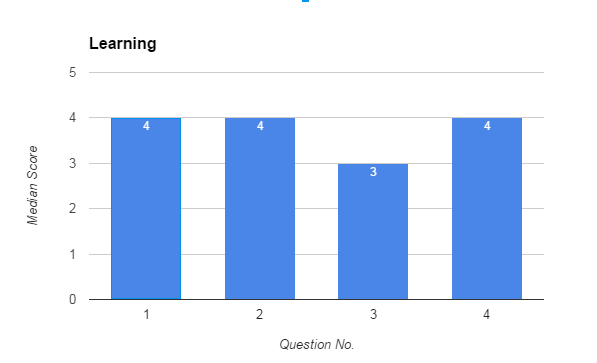
\includegraphics{./images/section2.png}}
\begin{figure}[h!]
  \centering
    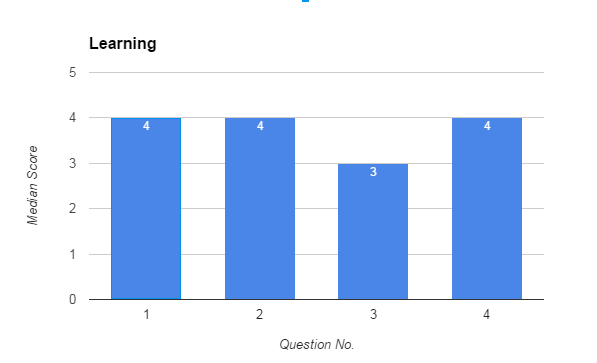
\includegraphics[width=0.5\textwidth]{./images/section2.png}
  \caption{Median score per question in Learning section}
  \label{fig:13}
\end{figure}

%{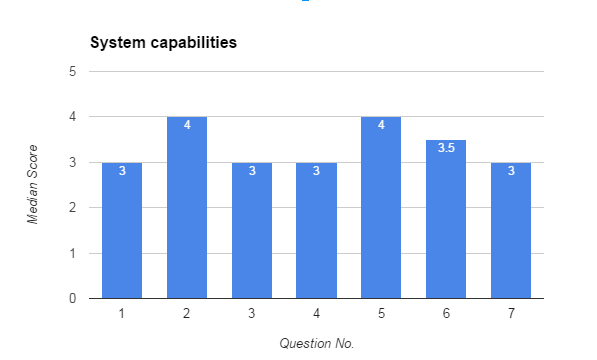
\includegraphics{./images/section3.png}}
\begin{figure}[h!]
  \centering
    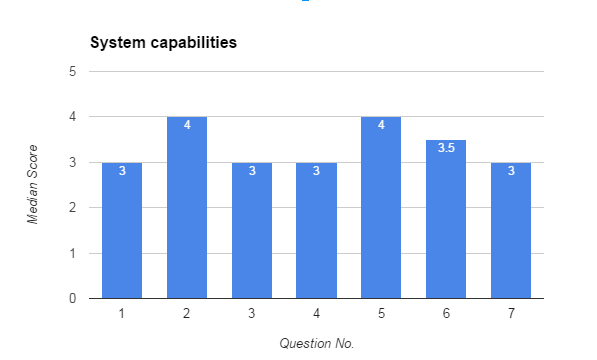
\includegraphics[width=0.5\textwidth]{./images/section3.png}
  \caption{Median score per question in  system capabilities  section }
  \label{fig:14}
\end{figure}

%{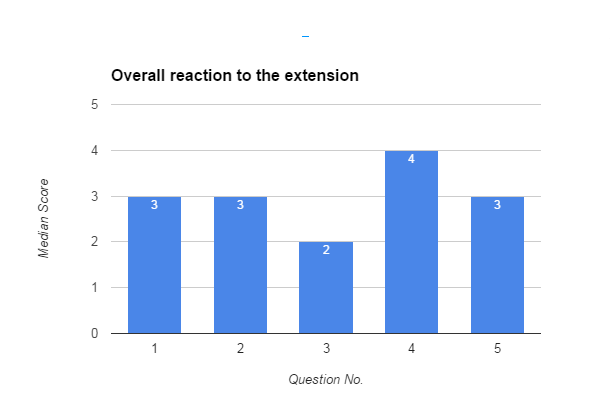
\includegraphics{./images/section4.png}}
\begin{figure}[h!]
  \centering
    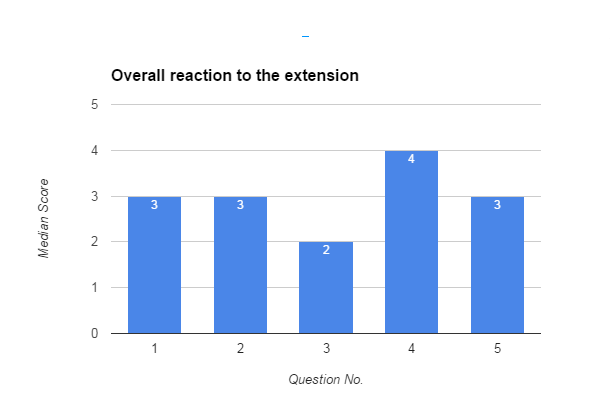
\includegraphics[width=0.5\textwidth]{./images/section4.png}
  \caption{Median score per question in Overall reaction to the extension section }
  \label{fig:15}
\end{figure}

From the data presented from the overall results of QUIS (see Figure ~\ref{fig:11}) the average score of 4.5 from the first section means that most of the respondents were satisfied by the consistency of the use of terms throughout extension, the error messages, and the position of messages on screen.  

Having  an average score of 3.8 out of 5 for the learnability means that it is not difficult but also not very easy.  However, it is worth noting that almost 70\% or  21 out of 30 participants had difficulty in learning to navigate a webpage using the extension. For the overall rating for learning to navigate webpages using eyeGalaw, almost half of the respondents had a difficulty (rating of 3 and below) than the respondents who rated eyeGalaw as easy to learn. 

The system capabilities section with an average score of 3.6 means that eyeGalaw had issues in it’s efficiency (see Figure ~\ref{fig:14}). This section evaluated its speed, flexibility to users and error handling. In terms of speed,  63.4\%  or 19 out of  30 of the respondents experienced a slow response to the actions such as scrolling up and down and  adjusting settings. From the 30 respondents, half of them agreed that eyeGalaw is designed for all kinds of users. But the overall usefulness of eyeGalaw in web page navigation was agreed as ‘useful’ (rating of 3 and above)  by 73.4\%  or  22 out of 30 respondents. Even if most of the respondents see it as useful in web page navigation, the issues in response speed and user type flexibility cannot be overlooked and should be addressed. 

Respondent’s overall reaction to the extension was also evaluated receiving an average median  score of 3. This means that most of the respondents reacted neutrally between strongly disagreeing and strongly  agreeing to the components being evaluated. The items include Difficult / Easy, Terrible / Wonderful, Frustrating / Satisfying,  Dull / Stimulating, and Rigid / Flexible. 

For the CSUQ, the questions were also categorized into two types namely: User-friendliness, and extension design efficiency. Questions 1 2,6,7,8,9,10, and 11 apply to user-friendliness; questions 3,4,5,12, and 13 concern to extension design efficiency. Similar with the procedure above, the average median scores by type are computed.

From the graph of average median score per section in CSUQ(see Figure ~\ref{fig:16}), data showed that the user-friendliness scored an average of 3.9 which means that the user interface of the application was satisfactory. The score of 2.9 in the extension design efficiency denotes that there are still problems in effectively navigating webpages using eyeGalaw. 
This may be attributed to the  difficulty of the respondents, as mentioned above, in learning to navigate a webpage using the extension. Another factor contributed to the problems in efficiency is the response speed of the extension, that is pointed in the discussion of system capabilities section above. 

%{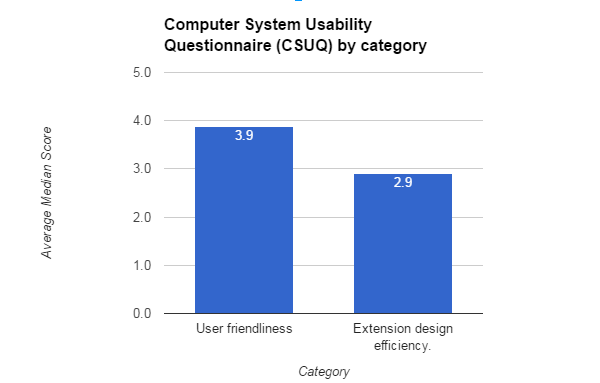
\includegraphics{./images/csuq.png}}
\begin{figure}[h!]
  \centering
    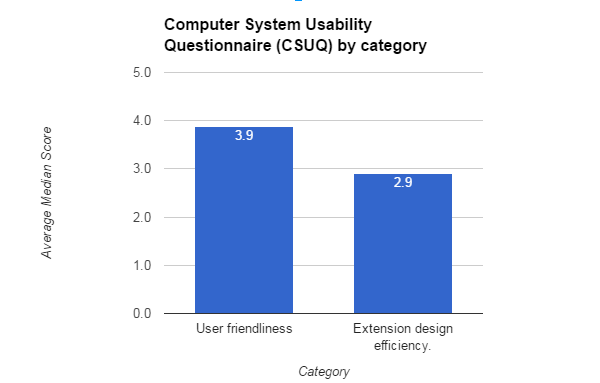
\includegraphics[width=0.5\textwidth]{./images/csuq.png}
  \caption{Average median score per section in CSUQ }
  \label{fig:16}
\end{figure}
\FloatBarrier
%{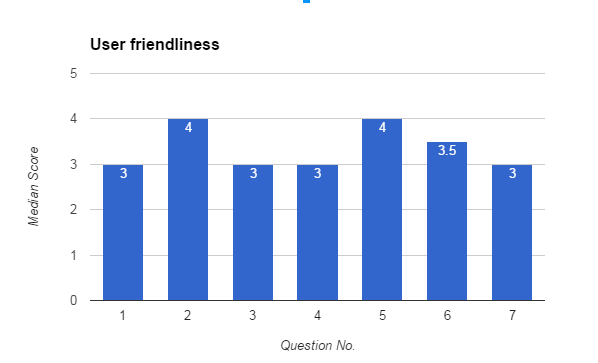
\includegraphics{./images/userfr.png}}
\begin{figure}[h!]
  \centering
    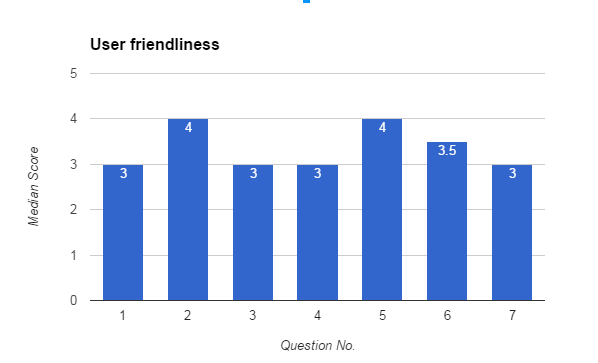
\includegraphics[width=0.5\textwidth]{./images/userfr.png}
  \caption{Median score per question in User-friendliness category }
  \label{fig:17}
\end{figure}
\FloatBarrier
%{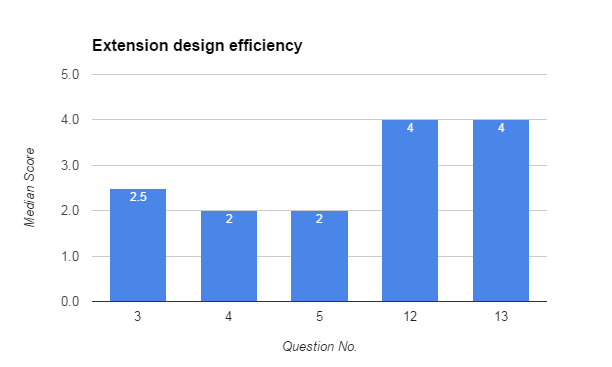
\includegraphics{./images/effiiciency.png}}
\begin{figure}[h!]
  \centering
    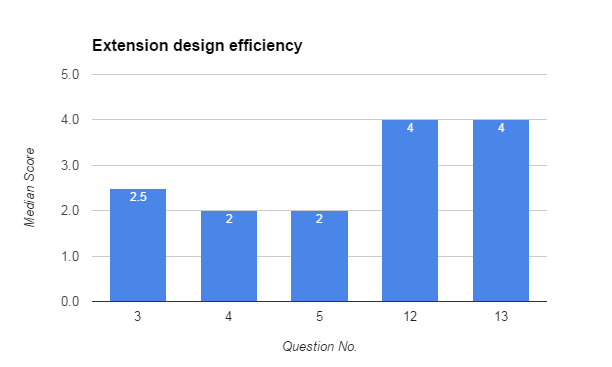
\includegraphics[width=0.5\textwidth]{./images/effiiciency.png}
  \caption{Median score per question in Extension design efficiency category }
  \label{fig:18}
\end{figure}
\FloatBarrier



\section {Conclusions and Future Work}

eyeGalaw, a Google chrome extension to navigate webpages using the eyes with the help of a web camera was successfully created. The user’s gaze location on the screen was successfully detected using an ordinary webcam securely. Gaze controlled navigation method was successfully incorporated with the normal click and scroll browsing.  Functions were successful with some reservations.  Although problems on speed and learnability of the extension hinder its efficiency, the overall usefulness of eyeGalaw in web page navigation is still commendable. 

The extension was tested on simple websites consisting of mostly texts and pictures only. The app was not tested on social media such as facebook, and twitter because there are elements such as facebook chat, and mostly website headers that cover eyeGalaw's controls. 

Possible improvements on the response speed and user-friendliness should be taken into consideration. Adding  in-application hints and a tutorial mode on how to operate eyeGalaw can possibly help ease the user's difficulty in learning to use the extension. Detecting elements in a webpage such as website headers, facebook chat sidebar, and other elements that may hinder the compatibility of eyeGalaw to websites should also be considered.  

This study has been an initial step from the inspiration of developing a google chrome extension to assist persons with locomotor problems and persons with disability. Improvements in the future can extend eyeGalaw’s capabilities and improve its functionalities for a wider set of users. This could revolutionize web page navigation that caters for everyone, even for people with special needs. 


% APPENDICES
\appendices

\section{Questions in Questionnaire for User Interface Satisfaction (QUIS)} 
\subsection {Terminology and system information}
\begin{enumerate}
\item Use of terms throughout system (Inconsistent/Consistent).
\item Terminilogy is intuitive (Never/Always).
\item Position of messages on screen (Inconsistent/Consistent).
\item Prompts for adjusting input in settings tab (Confusing/Clear).
\item Error messages (Helpful/Unhelpful).
\end {enumerate}


\subsection {Learning}
\begin{enumerate}
\item Overall rating for learning to navigate webpages using eyeGalaw (Difficult/Easy).
\item Learning to operate and adjust eyeGalaw settings (Difficult/Easy).
\item Learning to navigate a webpage by eyeGalaw  (Difficult/Easy).
\item Performing  tasks is straightforward i.e. scrolling up/down,  hide controls and disable scrolling. (Never/Always).
\item  Use of terms throughout system (Inconsistent/Consistent).
\end {enumerate}

\subsection {System capabilities}
\begin{enumerate}
\item Overall eyeGalaw speed (Too slow/Fast enough).
\item eyeGalaw startup speed (Too slow/Fast enough).
\item eyeGalaw speed in responding to the actions that a user does i.e. adjusting settings, navigation. (Too slow/Fast enough).
\item eyeGalaw  failure mechanisms: Errors can occur without warnings, Error messages are displayed correctly (Unreliable/Reliable).
\item eyeGalaw  failure mechanisms: Periodic restarts or refresh can help fix extension problems (Unreliable/Reliable).
\item eyeGalaw is designed for all levels of users (Never/Always).
\item Overall usefulness of eyeGalaw in web page navigation (Not Useful/ Very Useful).
\end {enumerate}

\subsection {Overall reaction to the extension}
\begin{enumerate}
\item Difficult / Easy
\item Terrible / Wonderful
\item Frustrating / Satisfying 
\item  Dull / Stimulating 
\item Rigid / Flexible
\end {enumerate}

\section{Questions in  Computer System Usability Questionnaire (CSUQ)}
The questions were rated from Strongly Disagree to Strong Agree
\subsection {User-friendliness}
\begin{enumerate}
\item  [1] Overall, I am satisfied with how easy it is to use eyeGalaw
\item [2] It was simple to use eyeGalaw
\item  [6] The information (such as online help, on-screen messages, and other documentation) provided with eyeGalaw is clear.
\item [7] It is easy to find the information I needed.
\item [8] The information provided for the system is easy to understand.
\item [9] The organization of information on the system screens is clear.
\item [10] The iterface of eyeGalaw is pleasant.
\item [11] I like using the interface of eyeGalaw.
\end {enumerate}

\subsection {Extension design efficiency}
\begin{enumerate}
\item  [3]  I can effectively navigate webpages using eyeGalaw.
\item  [4]  I can effectively complete my work using eyeGalaw.
\item  [5] I can effectively complete my work quickly  using eyeGalaw.
\item  [12]  eyeGalaw has all the functions and capabilities I expect it to have.
\item  [13] Overall, I am satisfied with eyeGalaw.
\end {enumerate}

% BIBLIOGRAPHY
\bibliographystyle{./IEEE/IEEEtran}
\bibliography{./cs190-ieee-Webgazer-rrl}
% \nocite{*}

% BIOGRAPHY
%\begin{biography}[{\includegraphics{./yourPicture.eps}}]{Christine Mae H. Juruena is BSCS student }
%Biography text here...
%\end{biography}


\end{document}
 
